\tableofcontents
\newpage
\section{Основные задачи администрирования в Windows}
\label{GL1}
Администрирование системы Windows осуществляется путём настройки групп пользователей, разграничения их полномочий и создания специальных скриптов управления.
\subsection{Цель Работы}
\begin{itemize}
    \item Настроить рабочую среду.
    \item Настроить учётные записи.
    \item Познакомиться с командной строкой.
    \item Создать скрипты Windows
\end{itemize}
\subsection{Ход работы}

Для начала установим, что данная лабораторная работа выполняется на операционной системе Windows 10 Education (рис. \ref{fig:winedu}). 

\begin{figure}[h!]
    \centering
    \begin{minipage}[p]{0.45\linewidth}
            \centering
            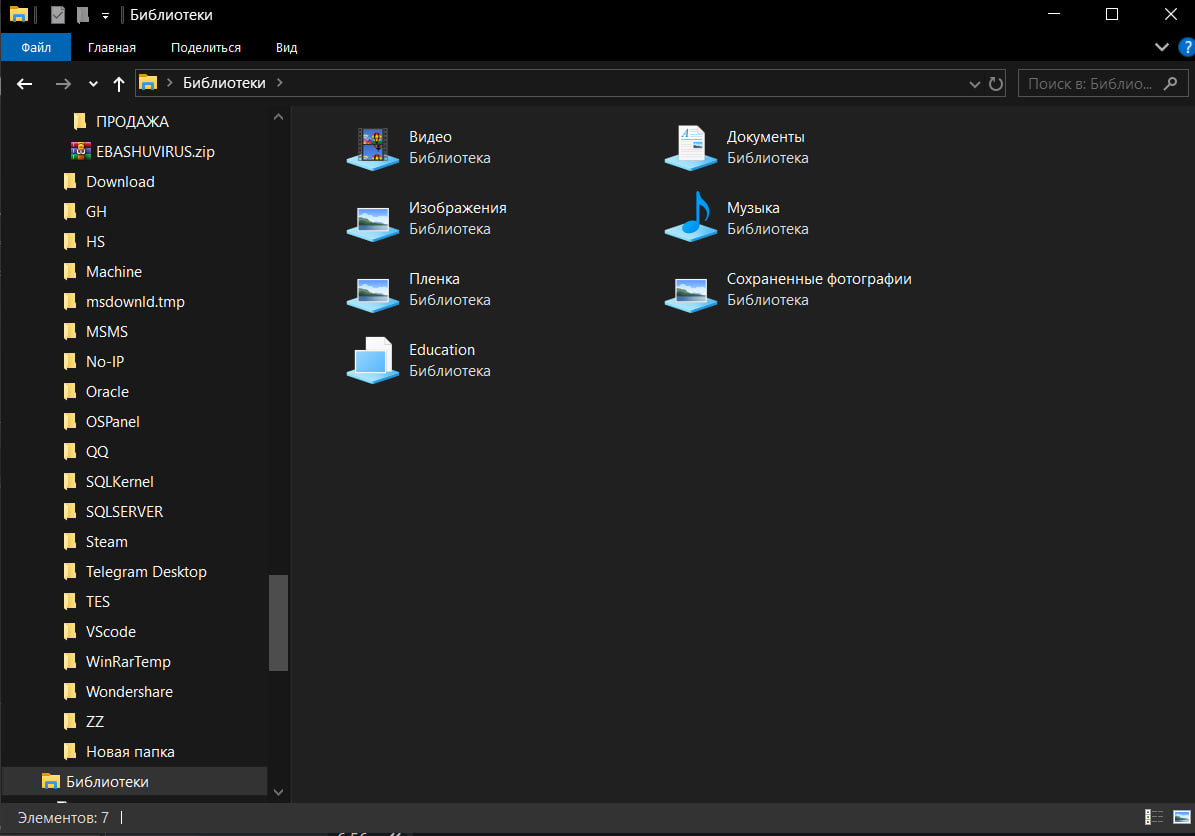
\includegraphics[width=1\linewidth]{Pic/lab1/photo_2025-05-21_08-15-00.jpg}
            \caption{Библиотеки пользователя.}
            \label{fig:bibuser}
    \end{minipage}
    \hfill
    \begin{minipage}[p]{0.45\linewidth}
            \centering
            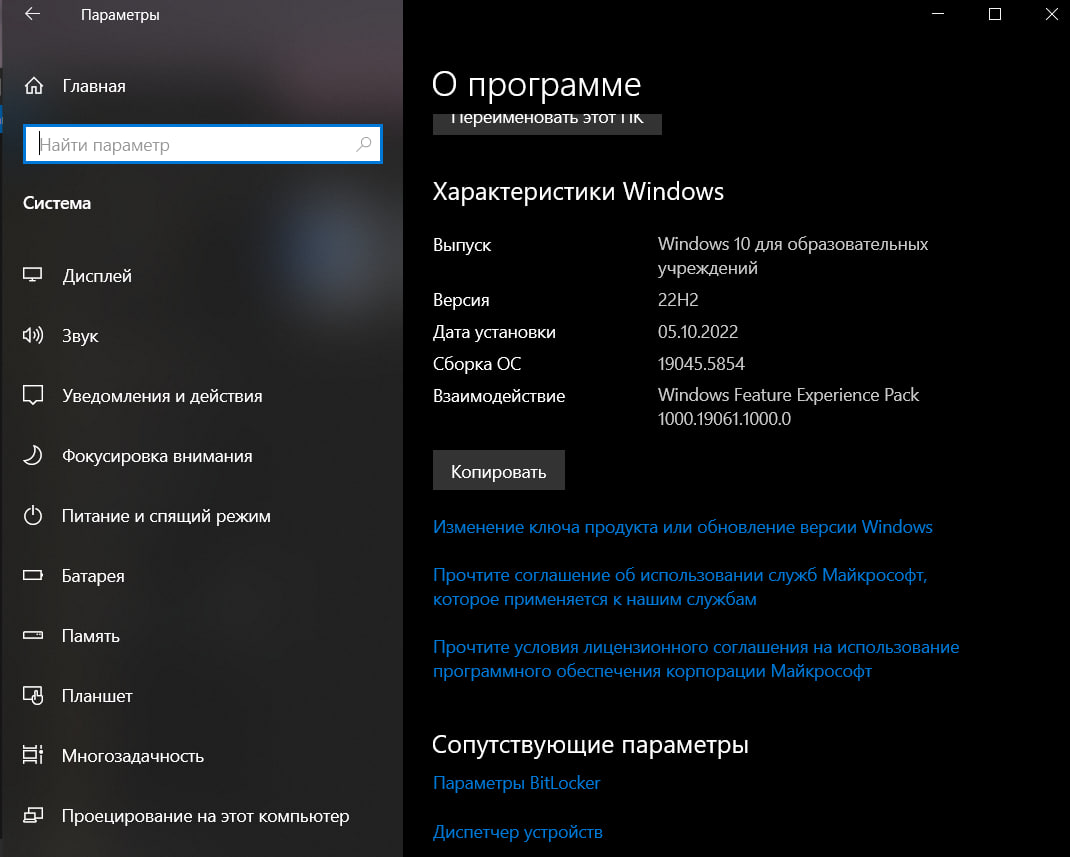
\includegraphics[width=0.9\linewidth]{Pic/lab1/photo_2025-05-21_08-14-59.jpg}
            \caption{Системные настройки.}
            \label{fig:winedu}
    \end{minipage}
    
\end{figure}

В системах Windows присутствует интерфейс Aero. В нём есть функции Aero Peek – быстро просмотреть рабочий стол, скрыв все окна; Aero Shake – свернуть все окна, кроме одного; Aero Snap – изменить размер окна.

При помощи программы Проводник открываем библиотеки пользователя и создаём ещё одну, нажав правую кнопку мыши и выбрав нужный пункт меню (рис. \ref{fig:bibuser}).

При помощи тех же средств управления внутри программы Проводник зададим ссылку на локальную директорию для данной библиотеки (рис. \ref{fig:bibinside}).
\begin{figure}[h!]
    \centering
    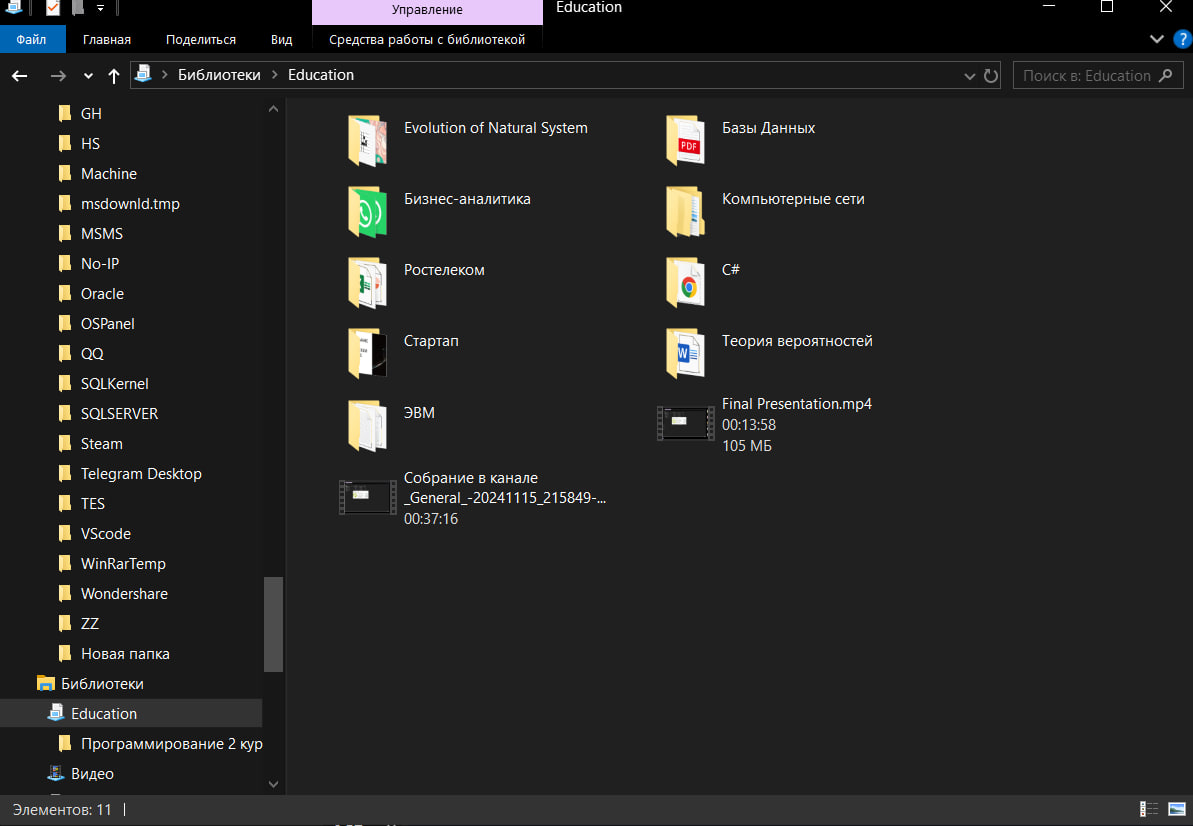
\includegraphics[width=0.5\linewidth]{Pic/lab1/photo_2025-05-21_08-15-02.jpg}
    \caption{Наполнение пользовательской библиотеки.}
    \label{fig:bibinside}
\end{figure}

Далее ознакомимся с пусковым меню. Здесь расположены все установленные в систему приложения, различные виджеты и другие полезные кнопки. Нажав правой кнопкой мыши на виджет, мы можем его закрепить или открепить (рис. \ref{fig:addvid}, \ref{fig:remvid}), изменить размер (рис. \ref{fig:scalevid}).

\begin{figure}[h!]
    \centering
    \begin{minipage}[p]{0.45\linewidth}
            \centering
            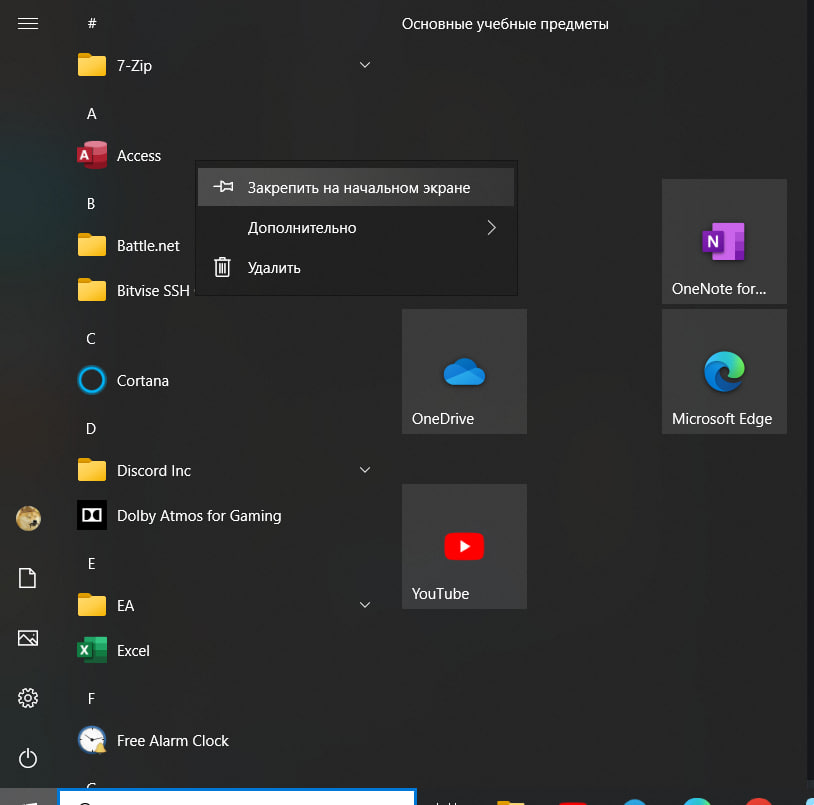
\includegraphics[width=1\linewidth]{Pic/lab1/photo_2025-05-21_08-15-05.jpg}
            \caption{Закрепление виджета.}
            \label{fig:addvid}
    \end{minipage}
    \hfill
    \begin{minipage}[p]{0.45\linewidth}
            \centering
            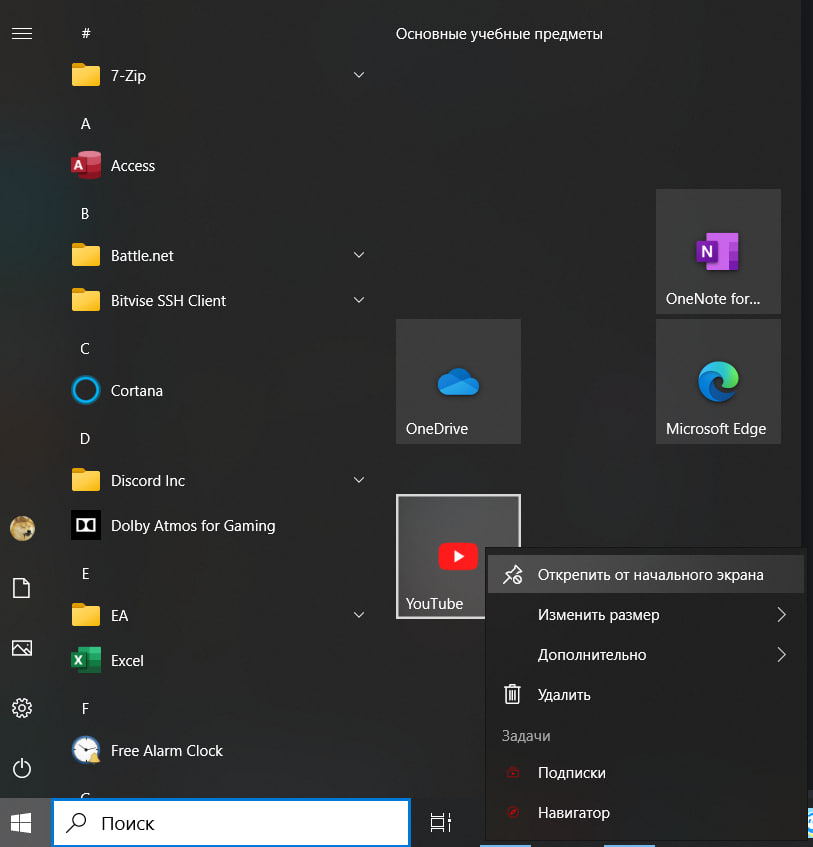
\includegraphics[width=0.95\linewidth]{Pic/lab1/photo_2025-05-21_08-15-07.jpg}
            \caption{Открепление виджета.}
            \label{fig:remvid}
    \end{minipage}
\end{figure}
\begin{figure}
    \centering
    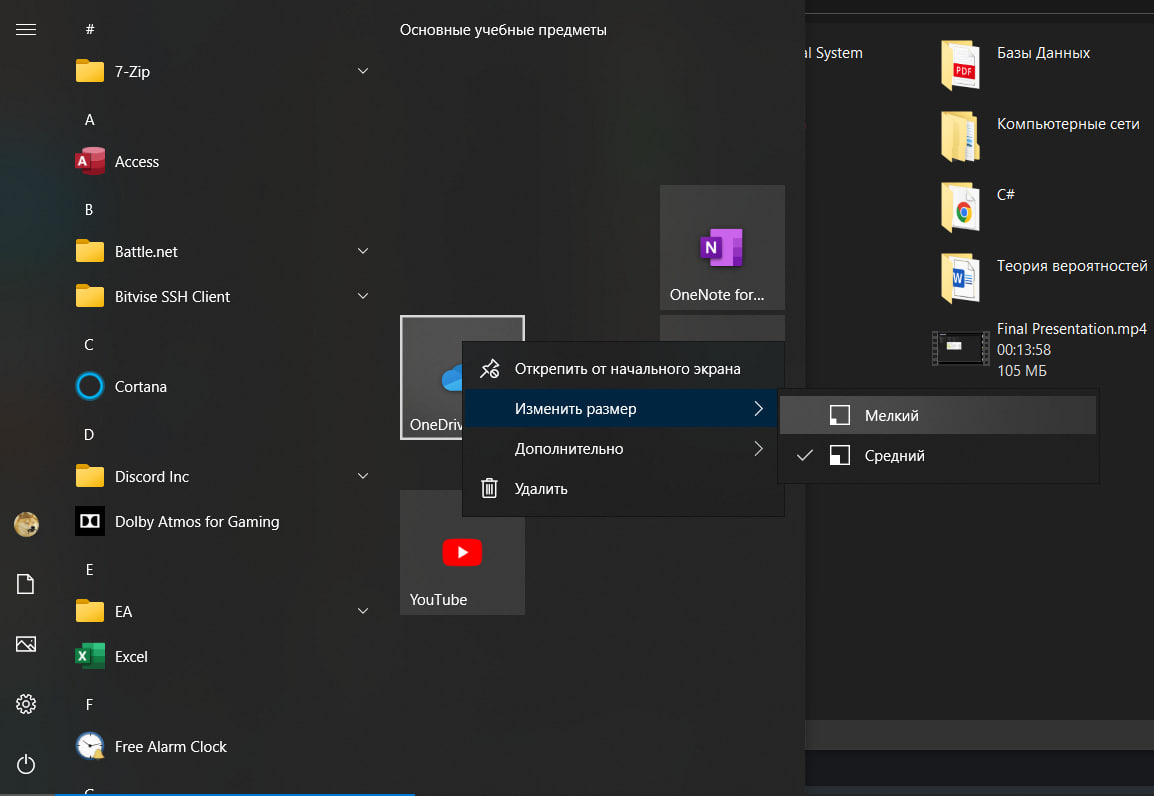
\includegraphics[width=0.5\linewidth]{Pic/lab1/photo_2025-05-21_08-15-04.jpg}
    \caption{Изменение размера.}
    \label{fig:scalevid}
\end{figure}

Помимо нативного управлдения через интерфейс, в Windows предусмотрено управление посредством горячих клавиш. Вот список некоторых из них:
\begin{table}[h!]
    \centering
    \caption{Таблица горячих клавиш}
    \label{tab:tab 1.1}
    \vspace{10}
    \begin{tabular}{|c|c|c|}
\hline
N&Сочетание клавиш&Действие\\
\hline
1&Win&Открыть/закрыть меню «Пуск»\\
\hline
2&Win + D&Свернуть/развернуть все окна и показать рабочий стол\\
\hline
3&Win + E&Открыть «Проводник»\\
\hline
4&Win + R&Открыть окно «Выполнить»\\
\hline
5&Win + Tab&Переключение между открытыми окнами\\
\hline
6&Win + Shift + Esc&Открыть диспетчер задач\\
\hline
7&Win + S&Открыть поиск Windows\\
\hline
    \end{tabular}
\end{table}

Для ориентации по приложения системы можно использовать пусковое меню, однако также существует полезная функция поиска (рис. \ref{fig:findapp}).
\begin{figure}
    \centering
    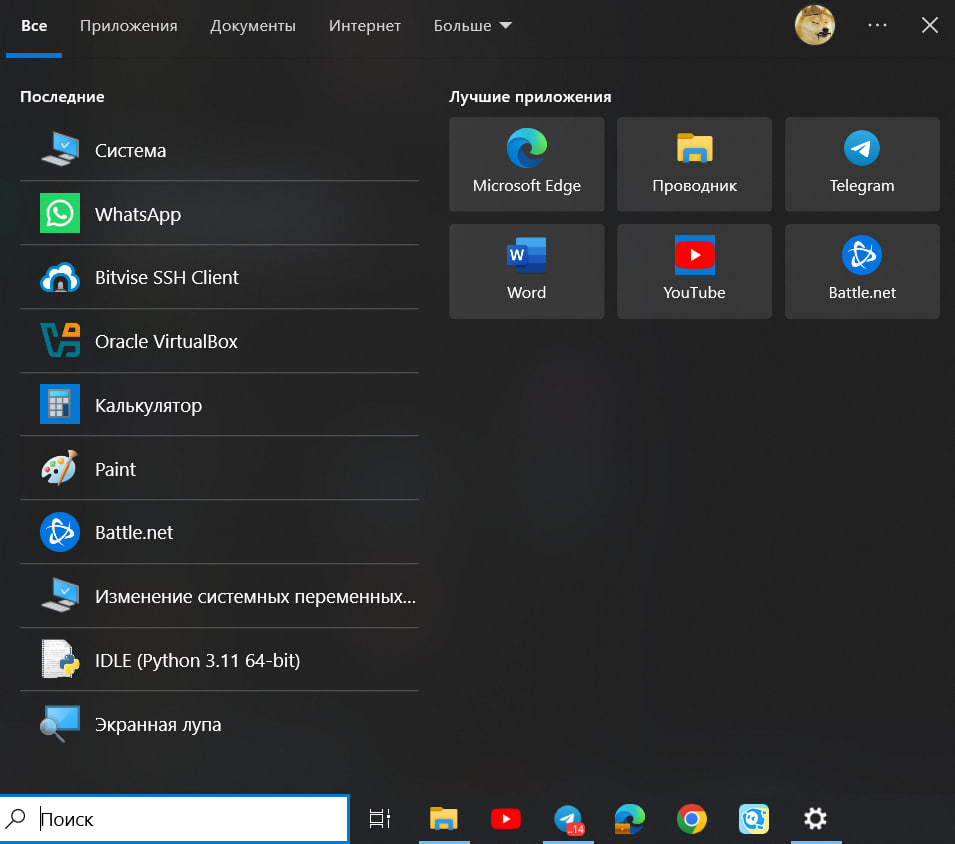
\includegraphics[width=0.5\linewidth]{Pic/lab1/photo_2025-05-21_08-15-11.jpg}
    \caption{Поиск приложений}
    \label{fig:findapp}
\end{figure}

Для быстрого обращения к приложениям используются ярлыки. Их можно создать при помощи виджетов пускового меню: перетащить на рабочий стол нужный виджет. Либо можно от при помощи правой кнопки мыши создать ярлык нужного файла.

\begin{figure}[h!]
    \centering
    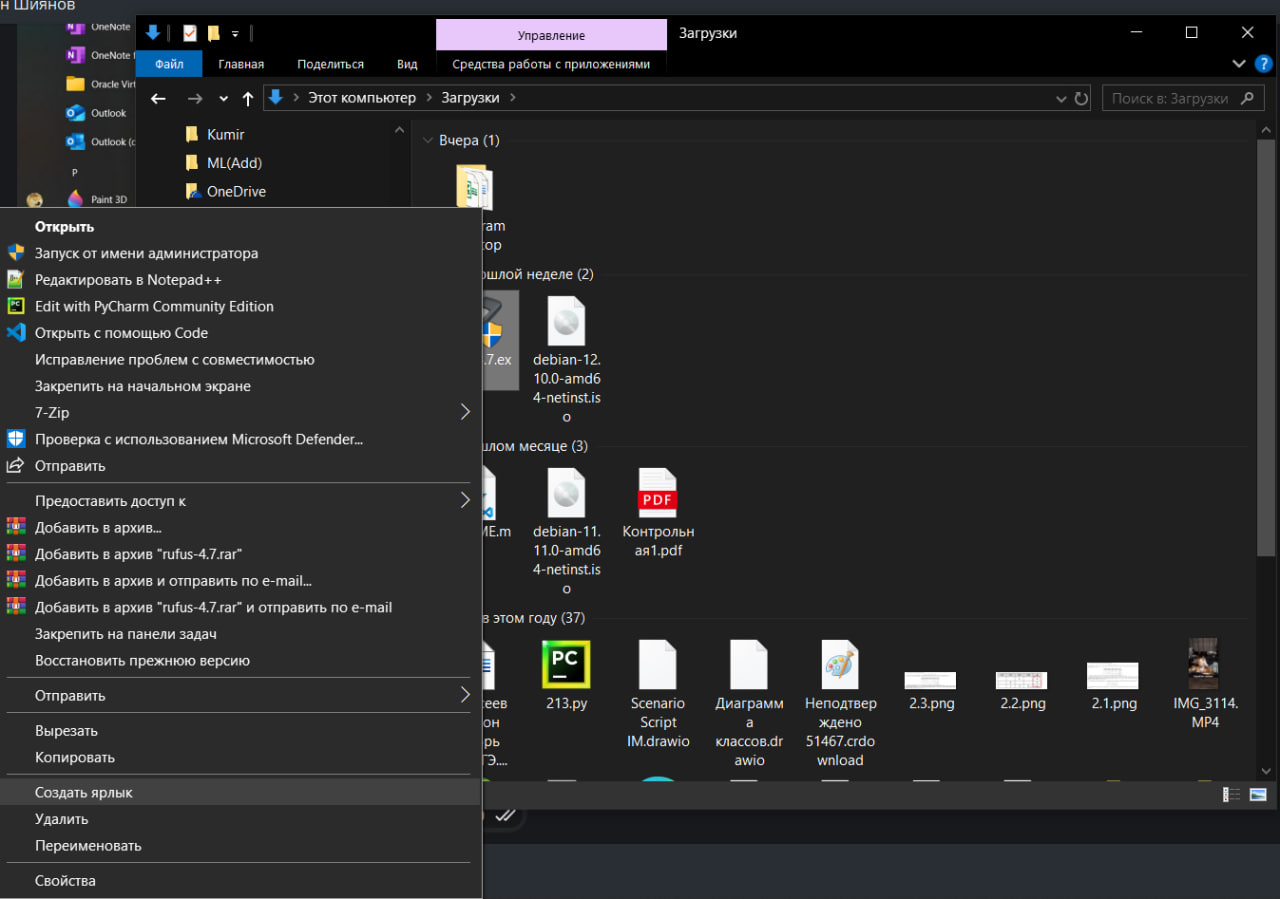
\includegraphics[width=0.5\linewidth]{Pic/lab1/photo_2025-05-21_08-15-12.jpg}
    \caption{Создание ярылка.}
    \label{fig:yrl}
\end{figure}

Далее перейдём к основным компонентам системы, службам и настройкам. Основные файлы системы, без которых она не может функционировать:
\begin{table}[h!]
    \centering
    \caption{Таблица компонент системы Windows}
    \label{tab:tab 1.1}
    \vspace{10}
    \begin{tabular}{|c|c|c|}
\hline
N&Название файла&Назначение\\
\hline
1&Bootmgr&Загрчик ОС\\
\hline
2&BCD&Параметры загрузки и сведения о доступных ОС\\
\hline
3&Winload.exe&Загружает ядро Windows и драйверы, необходимые для запуска\\
\hline
4&Ntoskrnl.exe&Ядро Windows – основной компонент операционной системы\\
\hline
5&Hal.dll&Аппаратно-абстрактный уровень – обеспечивает взаимодействие ОС с оборудованием\\
\hline
6&Smss.exe&Запускает подсистему сеанса и инициализирует пользовательский интерфейс\\
\hline
7&Csrss.exe&Подсистема клиент-сервер – управляет окнами, консолью и другими элементами\\
\hline
    \end{tabular}
\end{table}

В системе Windows существует программа Диспетчер задач. При помощи этой программы можно отслеживать процессы внутри системы и осуществлять контроль над ними. В нём существует функция автозагрузки. Через неё можно указать, какие приложения должны быть запущены вместе с загрузкой компьютера. Также это можно сделать через поиск специальной службы (рис. \ref{fig:autoload}). 

\begin{figure}[h!]
    \centering
    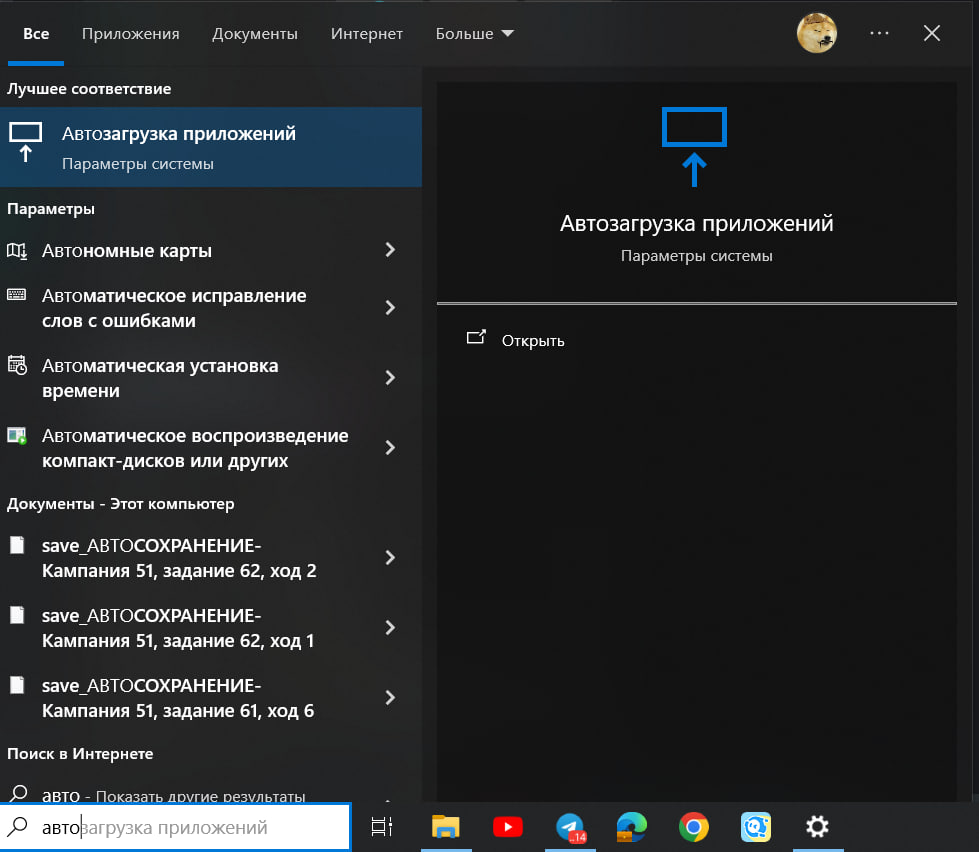
\includegraphics[width=0.5\linewidth]{Pic/lab1/photo_2025-05-21_08-15-14.jpg}
    \caption{Автозагрузка приложений.}
    \label{fig:autoload}
\end{figure}

Любым из этих двух способов мы попадём в окно служб, где присутствует список всех служб и параметры их работы (рис. \ref{fig:serv})

Когда мы разобрались с возможностями контроля системы, давайте посмотрим, как настраивать профили. Для этого при помощи сочетания win+R выполним запуск службы mmc (рис. \ref{fig:mmc}). 

\begin{figure}[h!]
    \centering
    \begin{minipage}[p]{0.45\linewidth}
    \centering
    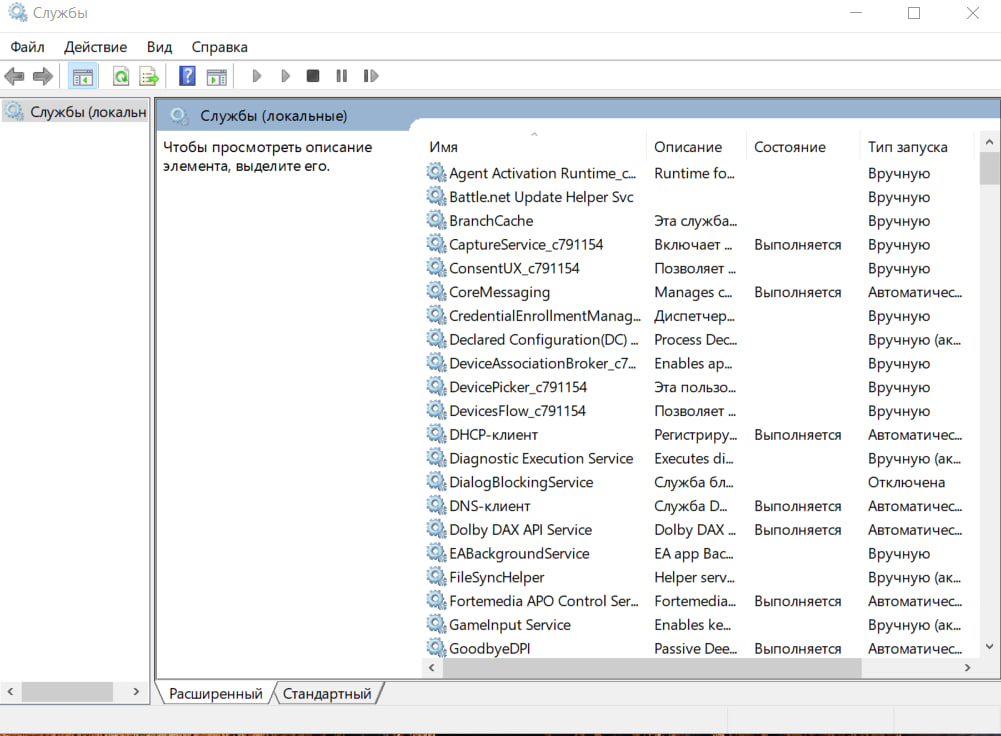
\includegraphics[width=0.7\linewidth]{Pic/lab1/photo_2025-05-21_08-15-15.jpg}
    \caption{Службы Windows.}
    \label{fig:serv}
    \end{minipage}
    \hfill
    \begin{minipage}[p]{0.45\linewidth}
    \centering
    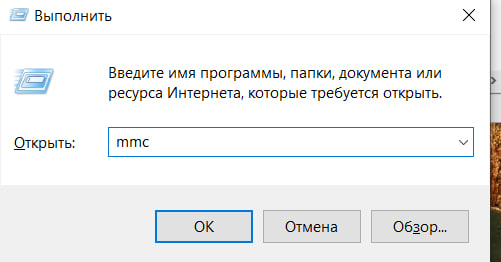
\includegraphics[width=1\linewidth]{Pic/lab1/photo_2025-05-21_08-15-17.jpg}
    \caption{Запуск mmc.}
    \label{fig:mmc}
    \end{minipage}
\end{figure}

В открывшемся окне нажимаем добавить оснастку. В этом меню указываем локального пользователя пользователя (рис. \ref{fig:UserCreat}). Далее справа наживаем на действие и выбираем создать нового пользователя.

Заполняем данные о пользователя как на примере. Учётную запись можно при этом создать отключённой. Это приведет к нескольким последствиям.
\begin{enumerate}
    \item Пользователь не сможет войти в систему до включения.
    \item Все файлы и настройки сохранятся, но доступ к ним будет ограничен.
    \item Программы и службы внутри учётной записи прекратят работу, кроме некоторых.
    \item Пользователю будет запрещено авторизоваться в сетевой среде, даже с других устройств.
\end{enumerate}
\begin{figure}
    \centering
    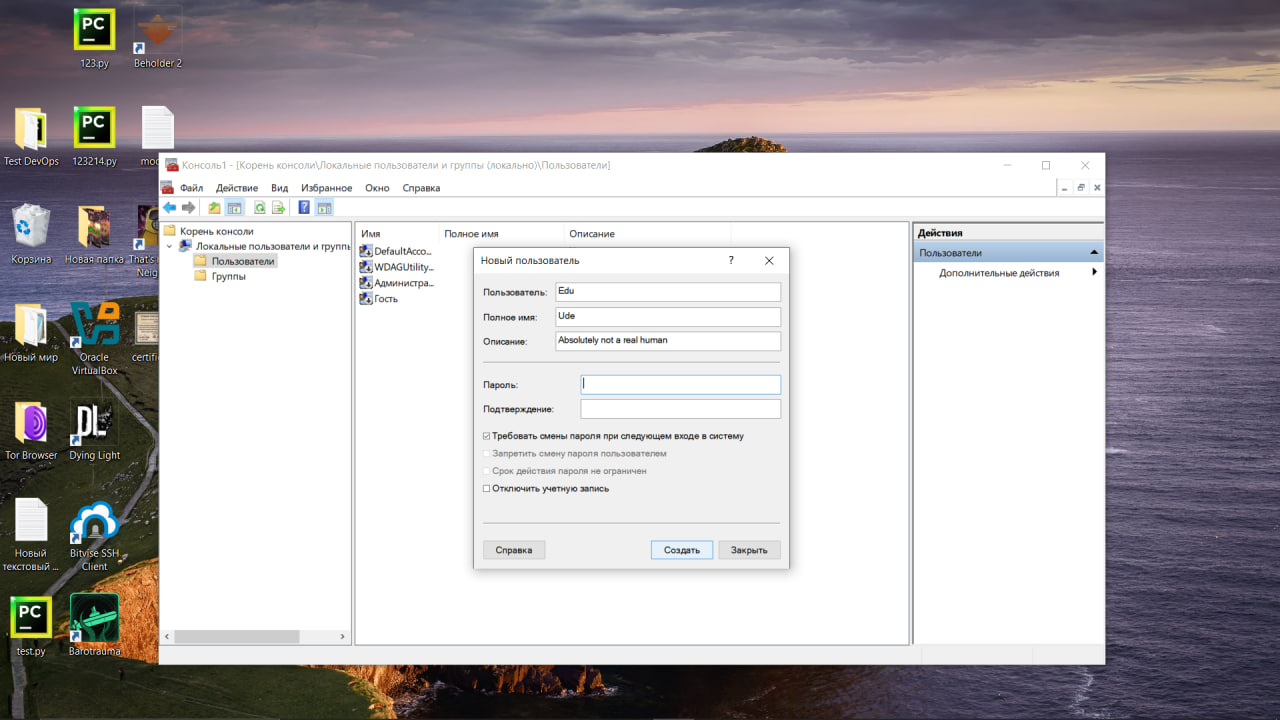
\includegraphics[width=0.5\linewidth]{Pic/lab1/photo_2025-05-21_08-15-22.jpg}
    \caption{Сведения о пользователе.}
    \label{fig:enter-label}
\end{figure}

\begin{figure}
    \centering
    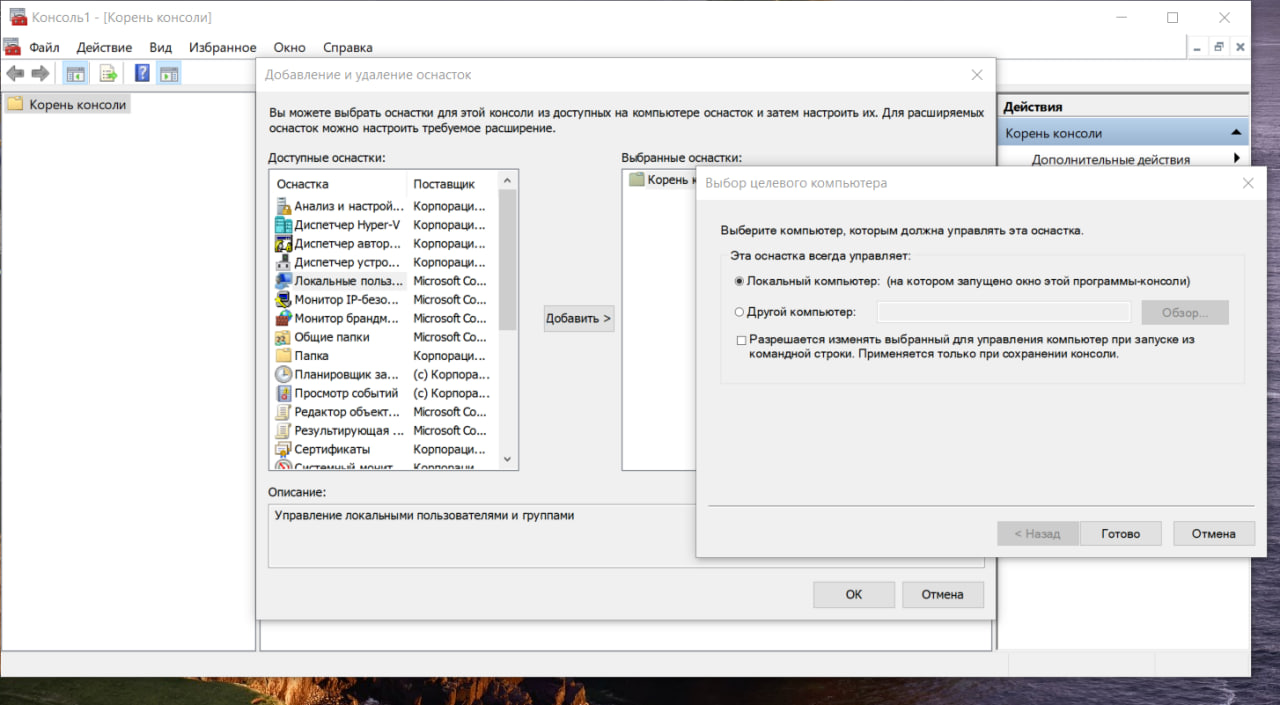
\includegraphics[width=0.5\linewidth]{Pic/lab1/photo_2025-05-21_08-15-19.jpg}
    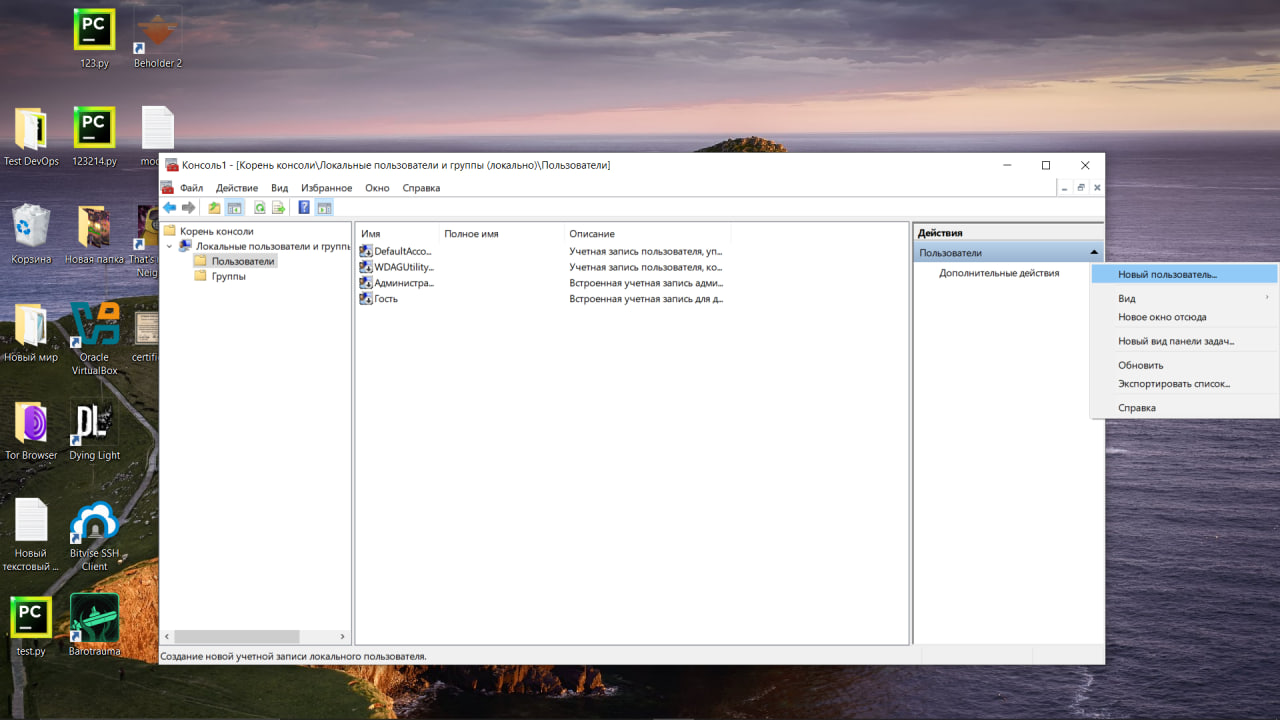
\includegraphics[width=0.5\linewidth]{Pic/lab1/photo_2025-05-21_08-15-20.jpg}
    \caption{Создание пользователя.}
    \label{fig:UserCreat}
\end{figure}

Отключенные учётные записи можно увидеть через оснастку Локальные пользователи и группы: через lusrmgr.msc или в свойствах учётных записей.

Далее создадим локальную группу. Для этого перейдём во вкладку ниже в том же окне, подписанную как группы. Справа, в окне действия, нажимаем на черный треугольник и выбираем создать группу. Следом откроется окно, где мы сможем указать название новой группы. Обязательно следует указать, какие пользователи войдут в эту группу. Выберем только что созданного пользователя (рис. \ref{fig:AddGroup}). 
\begin{figure}[h!]
    \centering
    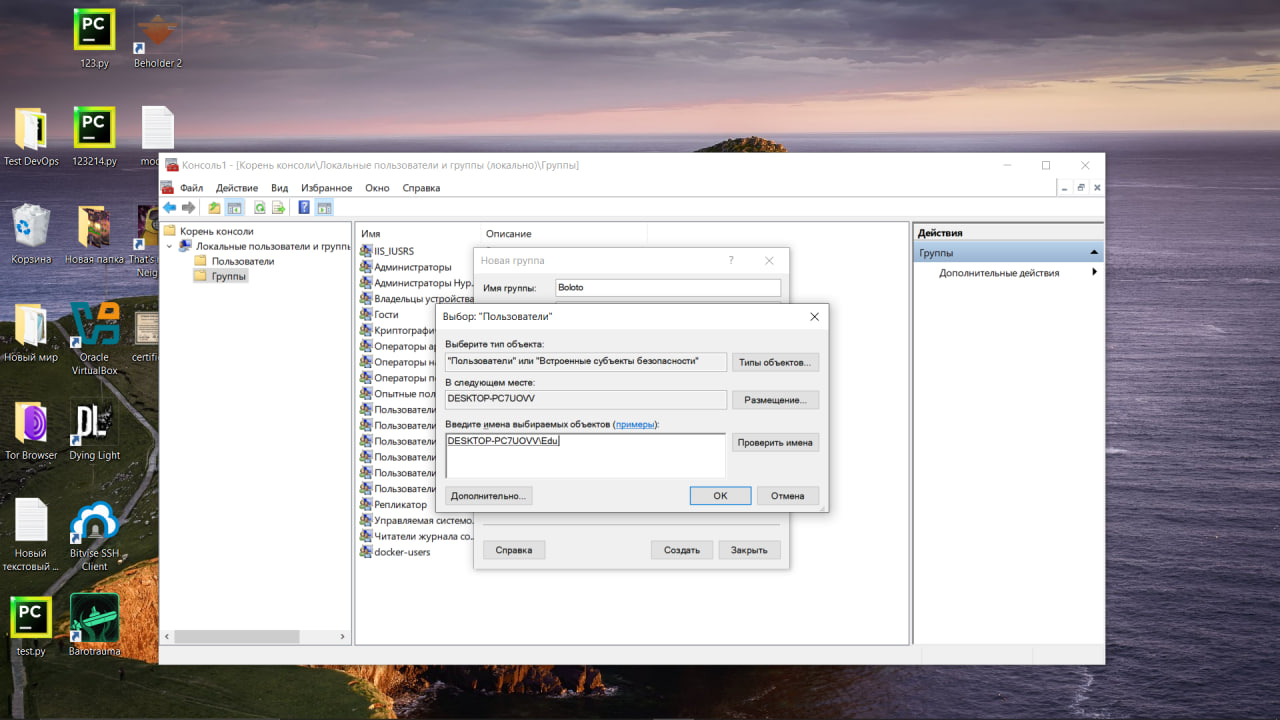
\includegraphics[width=0.5\linewidth]{Pic/lab1/photo_2025-05-21_08-15-25.jpg}
    \caption{Добавление пользователя в группу.}
    \label{fig:AddGroup}
\end{figure}

По стандарту в системе есть три пользователя: Admin - главный пользователь, его оль аналогична Super User в системах Linux; Guest - гостевая учётная запись с сильно ограниченными возможностями; User - стандартная учётная запись, используемая для повседневного взаимодействия с компьютером. Эти пользователи входят в следующие группы Admins, Guests, Users соответственно. Также могу существовать группа Power Users, пользователей с расширенными возможностями. При помощи утилиты lusrmgr.msc можно управлять группами пользователей. Добавлять их в группы, удалять из групп и т.п. 

В нашей системе существуют следующие пользователи: рис. \ref{fig:users}). По стандарту пользователи хранятся в директории C:/users/. Здесь можно увидеть стандартные папки профиля.

\begin{figure}[h!]
    \centering
    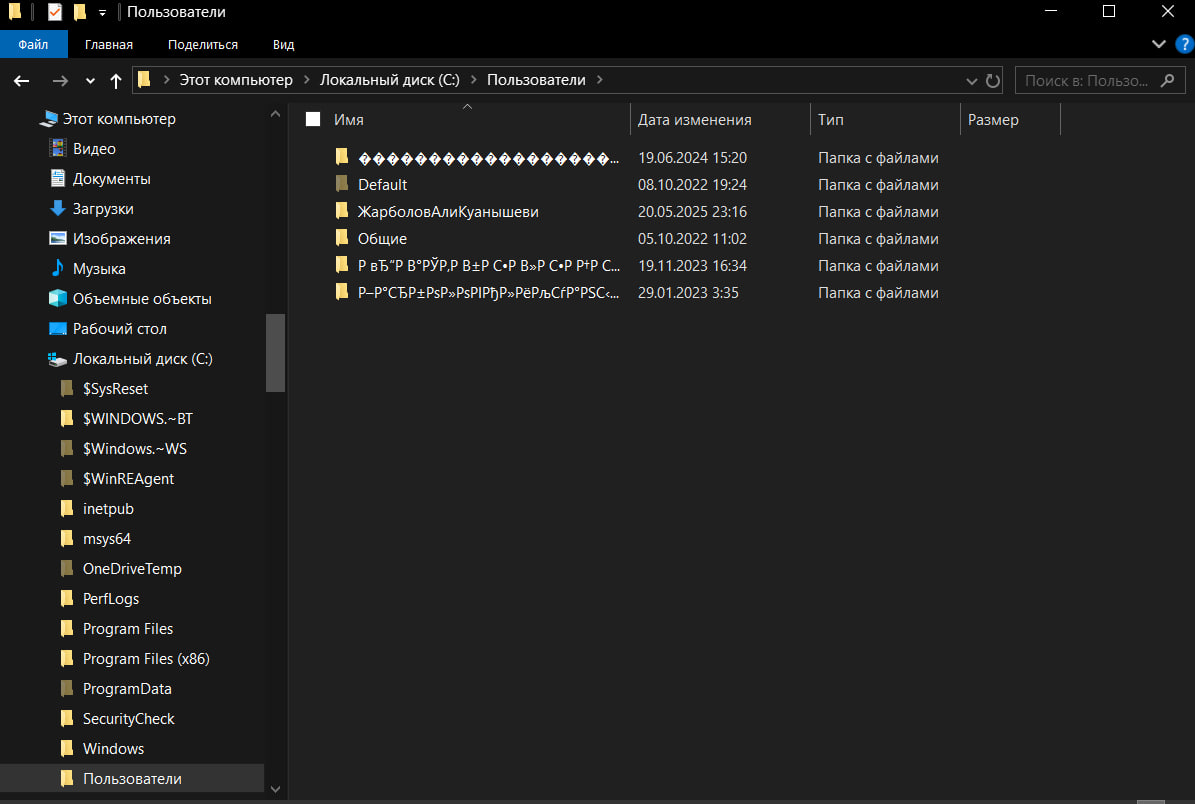
\includegraphics[width=0.5\linewidth]{Pic/lab1/photo_2025-05-21_08-15-26.jpg}
    \caption{Существующие пользователи.}
    \label{fig:users}
\end{figure}

\begin{table}[h!]
    \centering
    \caption{Стандартные папки пользователя.}
    \label{tab:tab 1.1}
    \vspace{10}
    \begin{tabular}{|l|l|}
\hline
Папка профиля&Назначение\\
\hline
Desktop&Рабочий стол пользователя\\
\hline
Documents&Документы\\
\hline
Downloads&Загруженные файлы\\
\hline
Pictures&Изображения\\
\hline
Videos&Видеофайлы\\
\hline
Music&Музыка\\
\hline
AppData&Скрытая системная папка с настройками программ\\
\hline
Favorites&Закладки Internet Explorer\\
\hline
Links&Ярлыки, которые отображаются в проводнике\\
\hline

    \end{tabular}
\end{table}

Все профили, о которых знает система, можно узнать при помощи утилиты System Properties Advanced. Она доступна из поиска или выполнением соответсвующей команды через меню Выполнить (рис. \ref{fig:PropAdvanced}). 

\begin{figure}[h!]
    \centering
    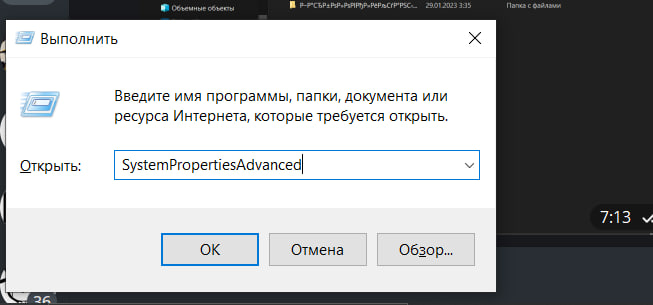
\includegraphics[width=0.5\linewidth]{Pic/lab1/photo_2025-05-21_08-15-28.jpg}
    \caption{Вызов расширенных настроек.}
    \label{fig:PropAdvanced}
\end{figure}

У нас появится окно Свойства системы. Здесь можно настраивать переменные среды, параметры восстановления системы, пользователей и т. д. Чтобы узнать о системных пользователях и изменить их тип, необходимо выбрать параметры в нужном пункте (рис. \ref{fig:usersparam}). Если нажать на кнопку, то можно и сменить тип пользователя (рис. \ref{fig:userstype}). Если тип перемещаемый, то настройка возможна через групповые политики. Если же тип обязательный, то переименование файла профиля с ntuser.dat на ntuser.man (это сделает пользователя обязательным). Через эту же утилиту осуществляется копирование пользователей, нужно только указать путь для копирования.

\begin{figure}[h!]
    \centering
    \begin{minipage}[p]{0.45\linewidth}
    \centering
    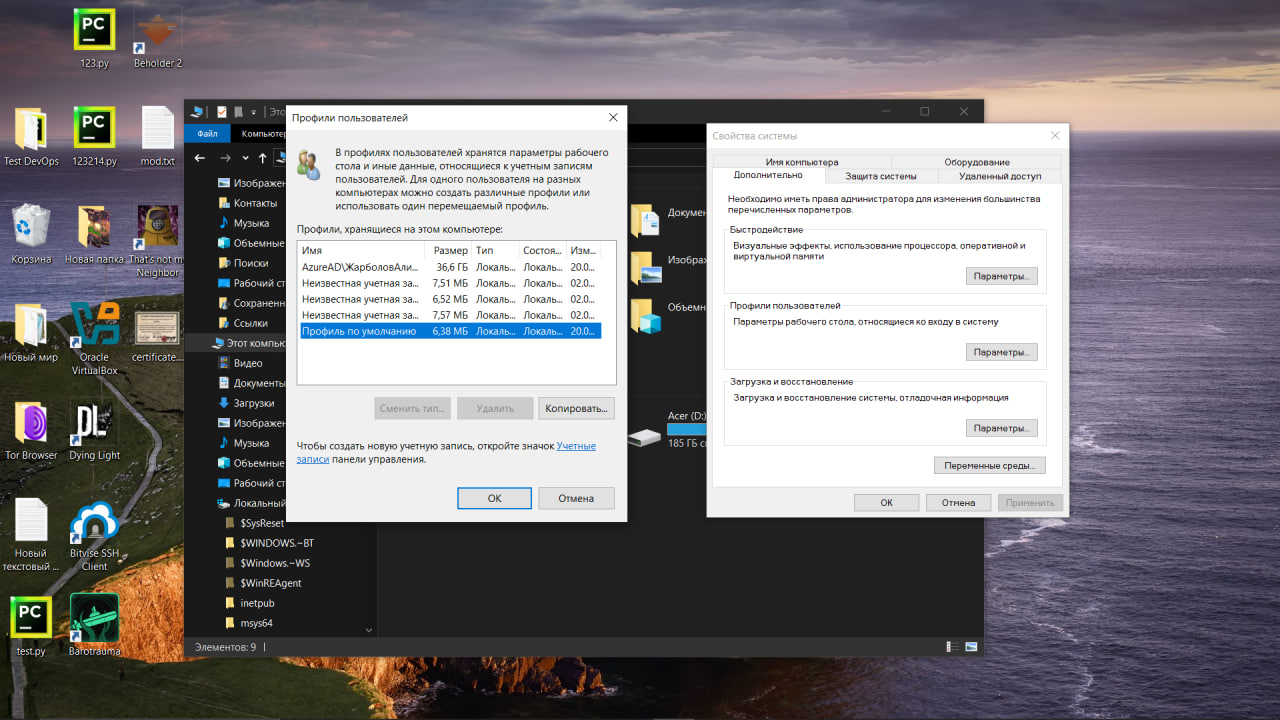
\includegraphics[width=1\linewidth]{Pic/lab1/photo_2025-05-21_08-15-31.jpg}
    \caption{Окно параметром пользователей.}
    \label{fig:usersparam}
    \end{minipage}
    \hfill
    \begin{minipage}[p]{0.45\linewidth}
    \centering
    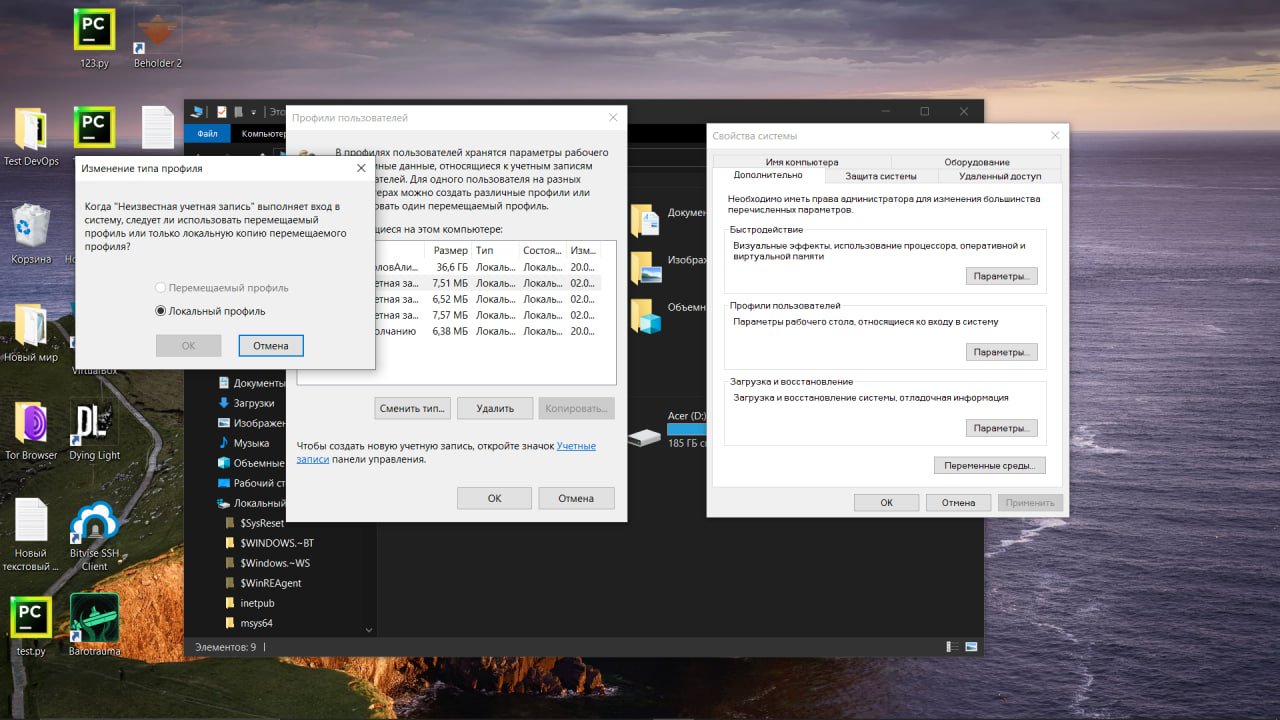
\includegraphics[width=1\linewidth]{Pic/lab1/photo_2025-05-21_08-15-29.jpg}
    \caption{Окно настройки типа пользователя.}
    \label{fig:userstype}
    \end{minipage}
\end{figure}

Помимо управления системой чеерез утилиты, контроль можно осуществлять через терминал. Вызов терминала возможен командой cmd в утилите Выполнить или через поиск. В терминале есть широкий инструментарий для работы с системой. Давайте перечислим некоторые основные команды:
\begin{figure}[h!]
    \centering
    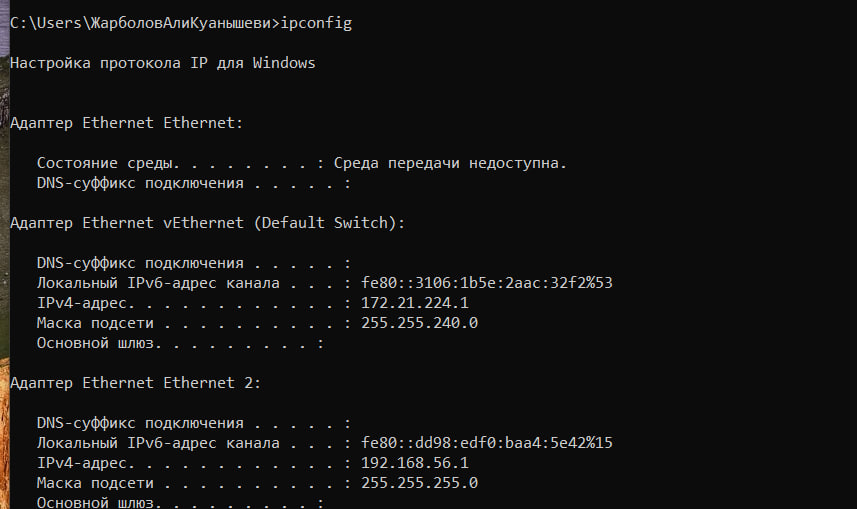
\includegraphics[width=0.5\linewidth]{Pic/lab1/photo_2025-05-21_08-15-33.jpg}
    \caption{Команда ipconfig: показывает все сетевые интерфейсы.}
    \label{fig:enter-label}
\end{figure}

\begin{figure}[h!]
    \centering
    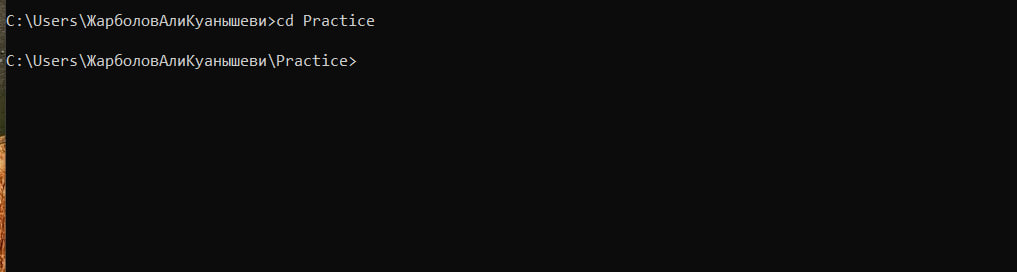
\includegraphics[width=0.5\linewidth]{Pic/lab1/photo_2025-05-21_08-15-34.jpg}
    \caption{Команда cd: осуществляет переход по указанному пути.}
    \label{fig:enter-label}
\end{figure}

\begin{figure}[h!]
    \centering
    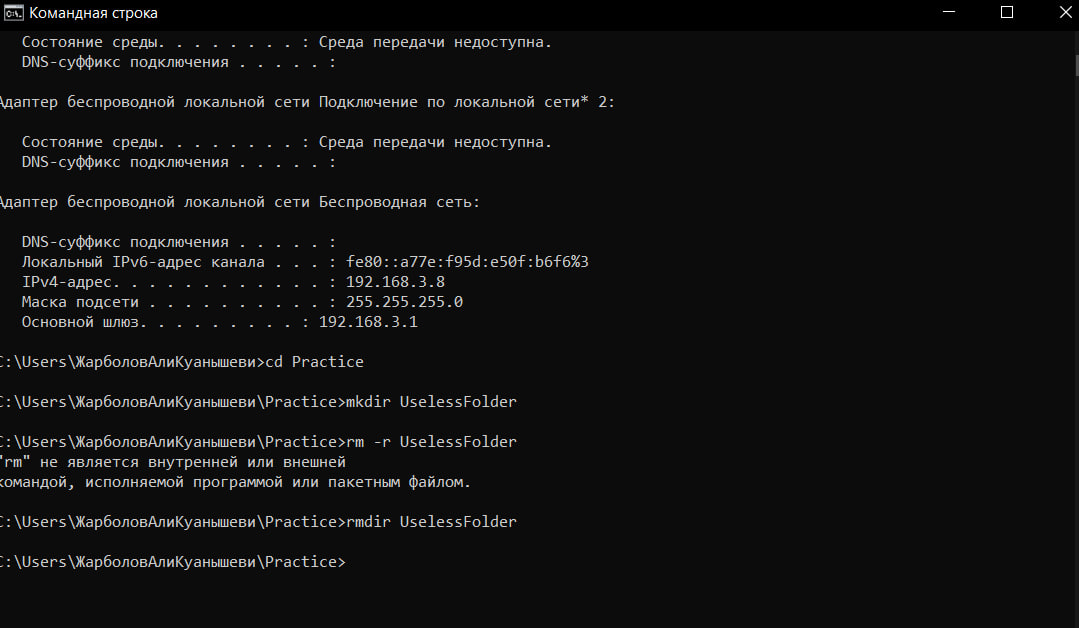
\includegraphics[width=0.5\linewidth]{Pic/lab1/photo_2025-05-21_08-15-36.jpg}
    \caption{Команды mkdir и rmdir: создаёт/удаляет директорию по указанному пути.}
    \label{fig:enter-label}
\end{figure}

\begin{figure}[h!]
    \centering
    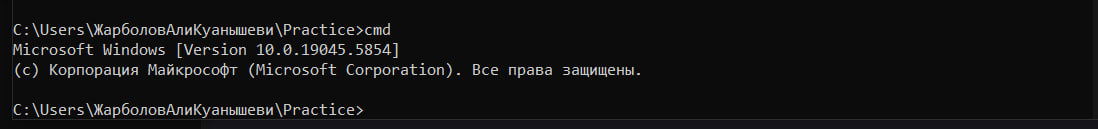
\includegraphics[width=0.5\linewidth]{Pic/lab1/photo_2025-05-21_08-15-38.jpg}
    \caption{Команда cmd: возвращает сведения о системе.}
    \label{fig:enter-label}
\end{figure}

\begin{figure}[h!]
    \centering
    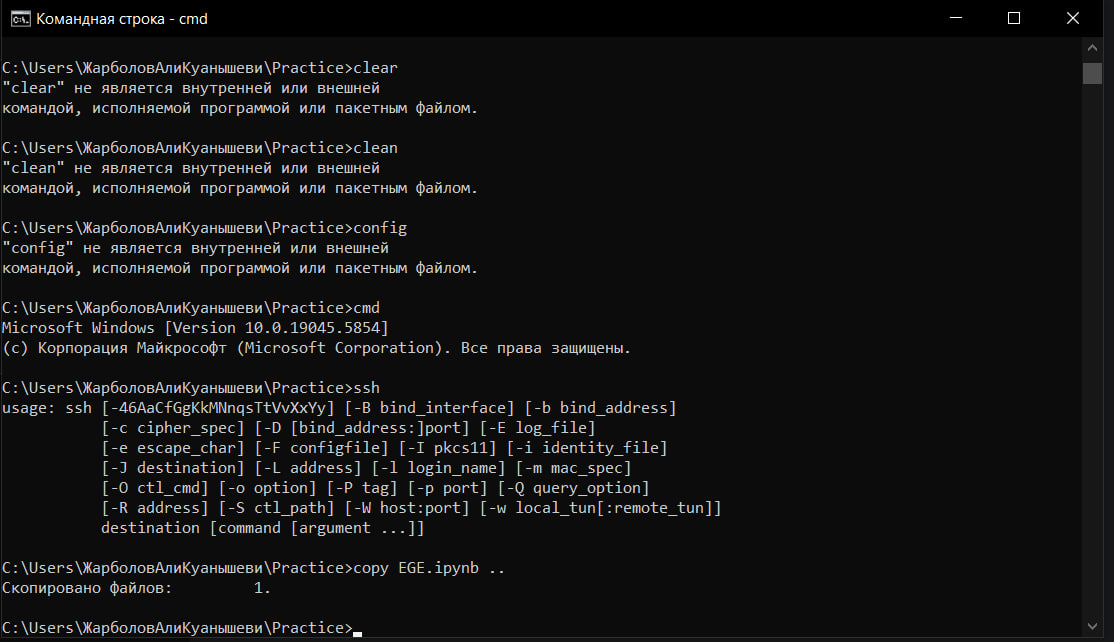
\includegraphics[width=0.4\linewidth]{Pic/lab1/photo_2025-05-21_08-15-40.jpg}
    \caption{Команда copy: копирует файл в указанное место на компьютере.}
    \label{fig:enter-label}
\end{figure}

\begin{figure}[h!]
    \centering
    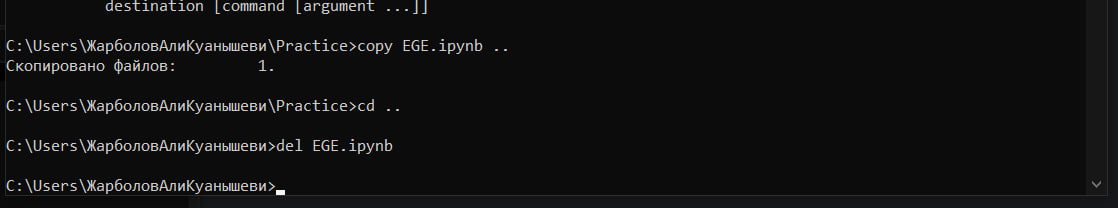
\includegraphics[width=0.5\linewidth]{Pic/lab1/photo_2025-05-21_08-15-41.jpg}
    \caption{Команда del: удаляет файл по указанному пути.}
    \label{fig:enter-label}
\end{figure}

\begin{figure}[h!]
    \centering
    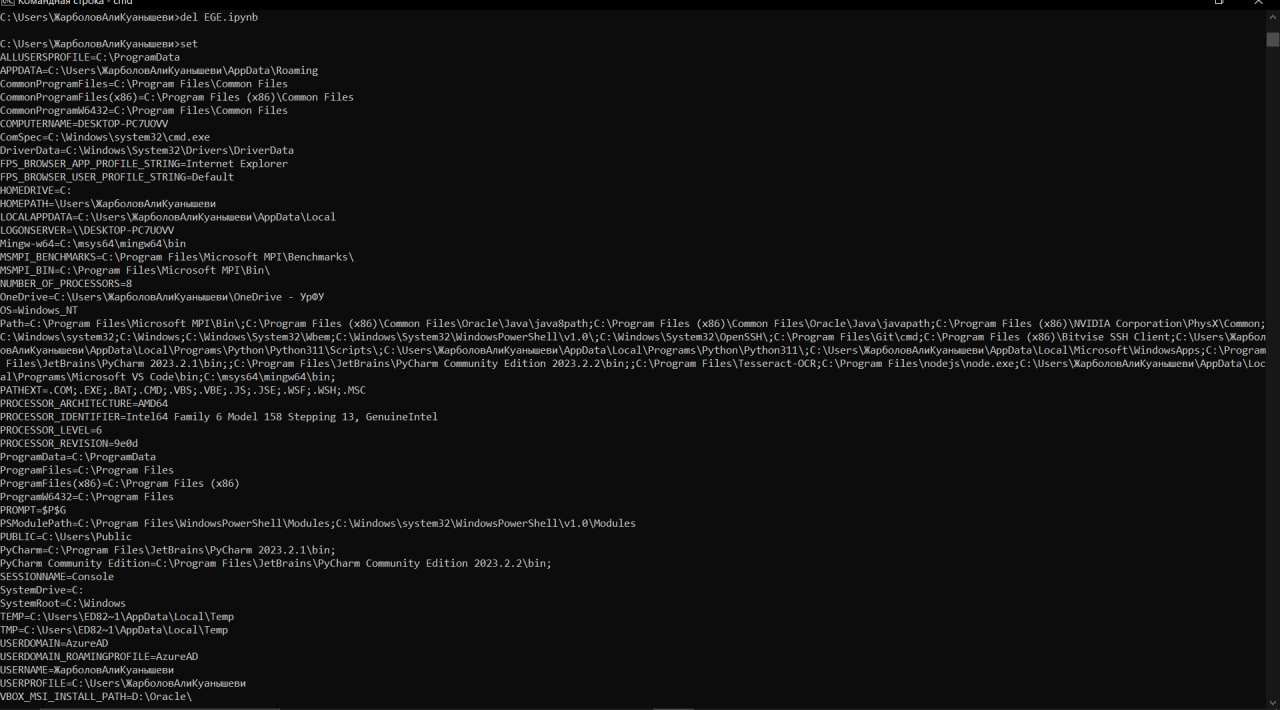
\includegraphics[width=0.5\linewidth]{Pic/lab1/photo_2025-05-21_08-15-43.jpg}
    \caption{Команда set: создаёт переменные среды.}
    \label{fig:set}
\end{figure}

Переменные среды весьма полезная функция Windows. Она позволяет указывать исполняемые скрипты/программы и другое ПО, которые могут быть вызваны из терминала. Переменные среды можно задать двумя способами. Первый способ - использовать специальную команду терминала (рис. \ref{fig:set}). Второй способ - использовать утилиту Свойства системы (рис. \ref{fig:usersparam}). Чтобы создать новую переменную, необходимо выбрать соответсвующий пункт в параметрах, далее нажать кнопку Создать (рис. \ref{fig:varenv}). Создав её, мы можем спокойно обращаться к заранее записанной директории просто по имени переменной, как на рисунке \ref{fig:varenvcall}.

\begin{figure}[h!]

\end{figure}
\begin{figure}[h!]
    \centering
    \begin{minipage}[p]{0.45\linewidth}
    \centering
    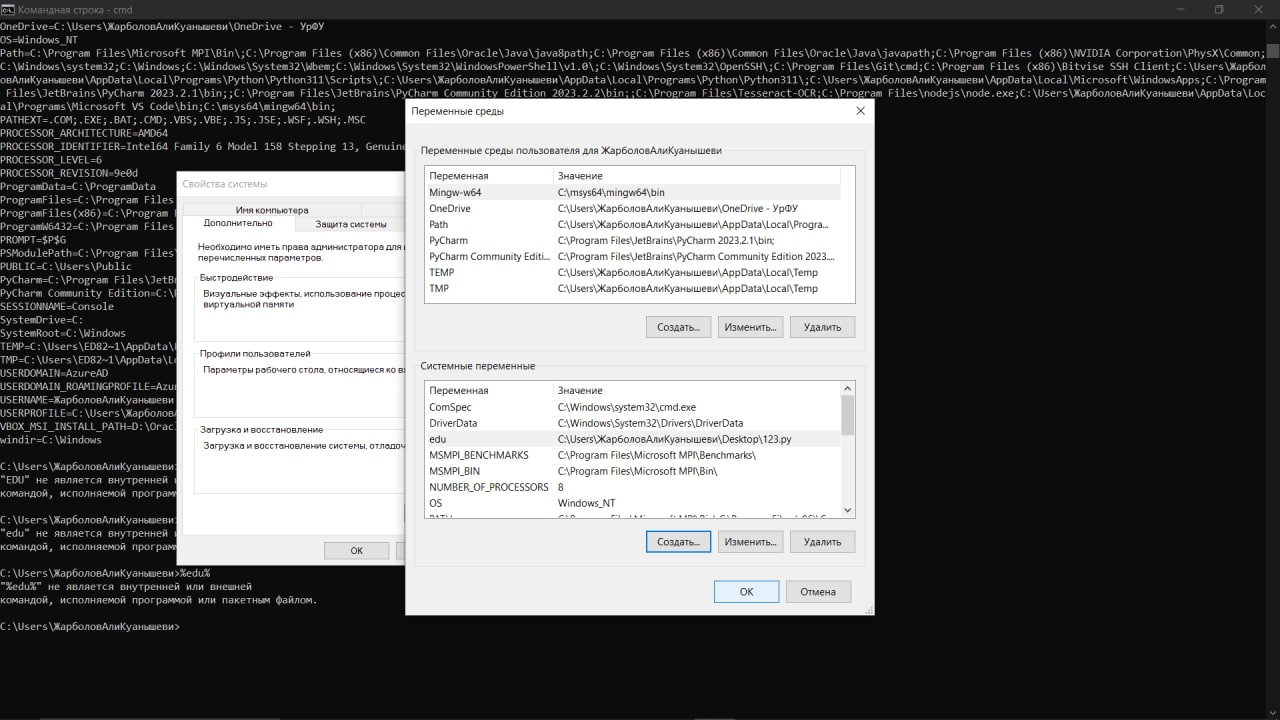
\includegraphics[width=1\linewidth]{Pic/lab1/photo_2025-05-21_08-15-44.jpg}
    \caption{Создание переменной среды.}
    \label{fig:varenv}
    \end{minipage}
    \hfill
    \begin{minipage}[p]{0.45\linewidth}
    \centering
    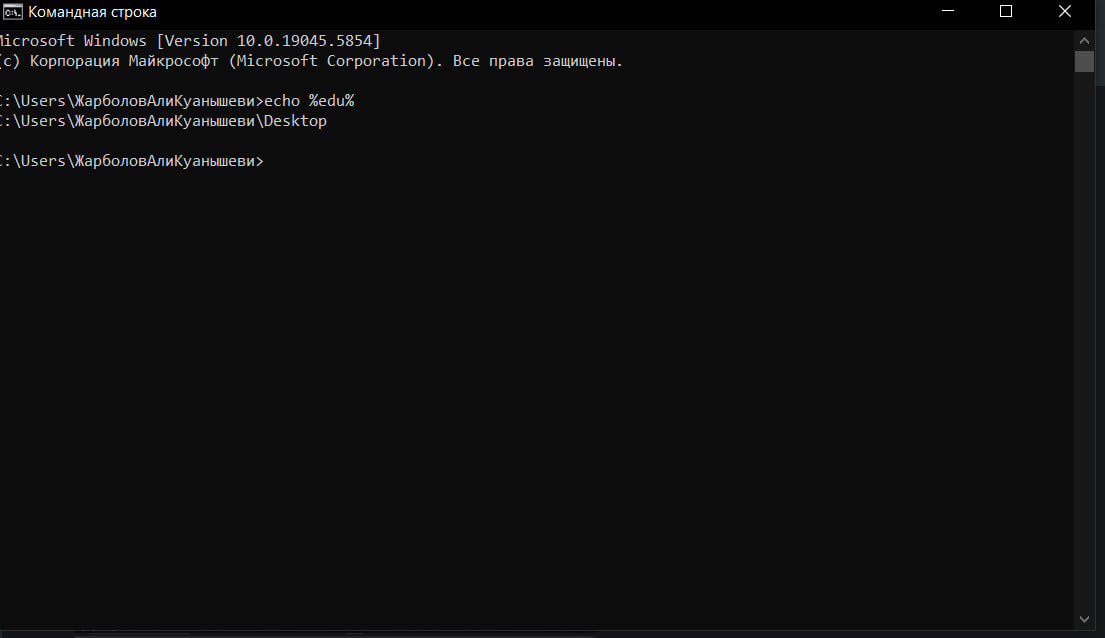
\includegraphics[width=1\linewidth]{Pic/lab1/photo_2025-05-21_08-15-46.jpg}
    \caption{Вызов переменной среды.}
    \label{fig:varenvcall}
    \end{minipage}
\end{figure}

В Windows существуют так называемые командные файлы. Это программы, написанные на специальном языке командной оболочки, напоминающим bash. Давайте создадим несколько скриптов. Для этого достаточно создать обычный текстовый документ, в котором надо написать исполняемую программу. Можно при этом указать расширение .bat или .cmd, впрочем это необязательно.

Давайте напишем программу для копирования файлов через командную оболочку.

\begin{verbatim}
        @echo off
        setlocal enabledelayedexpansion
        :: проверка того, что переданы файлы
        if "%~1"=="" (
            echo Error: you have to add at least one file extension for copying.
            exit /b 1
        )
        :: установим место копирования
        set "backup_dir=D:\documents\trash"
        if not exist "%backup_dir%" (
            mkdir "%backup_dir%"
        )
        :: метка начала алгоритма
        :loop
        if "%~1"=="" goto endloop
        set "ext=%~1"
        if "!ext:~0,1!"=="." set "ext=!ext:~1!"
        set "ext_dir=%backup_dir%\!ext!"
        if not exist "!ext_dir!" (
            mkdir "!ext_dir!"
        )
        :: цикл копирования подходящих файлов
        for /r %%f in (*.!ext!) do (
            copy "%%f" "!ext_dir!" >nul
        )
        shift
        goto loop
        :: метка конца алгоритма
        :endloop
        echo Copying is done.
        exit /b 0

\end{verbatim}

Как это выглядит в текстовом документе можно посмотреть на рисунке \ref{fig:CopeScript}. Запуск осуществляется через PowerShell. Возможно и через CMD, но придётся перейти в директорию со скриптом или указывать полный путь до файла. Для запуска скрипта достаточно просто указать запускаемый файл в терминале (рис. \ref{fig:RunCopy}). В указанной директории (рис. \ref{fig:CopyResult}) видим, что копирование прошло успешно.

\begin{figure}[h!]
    \centering
    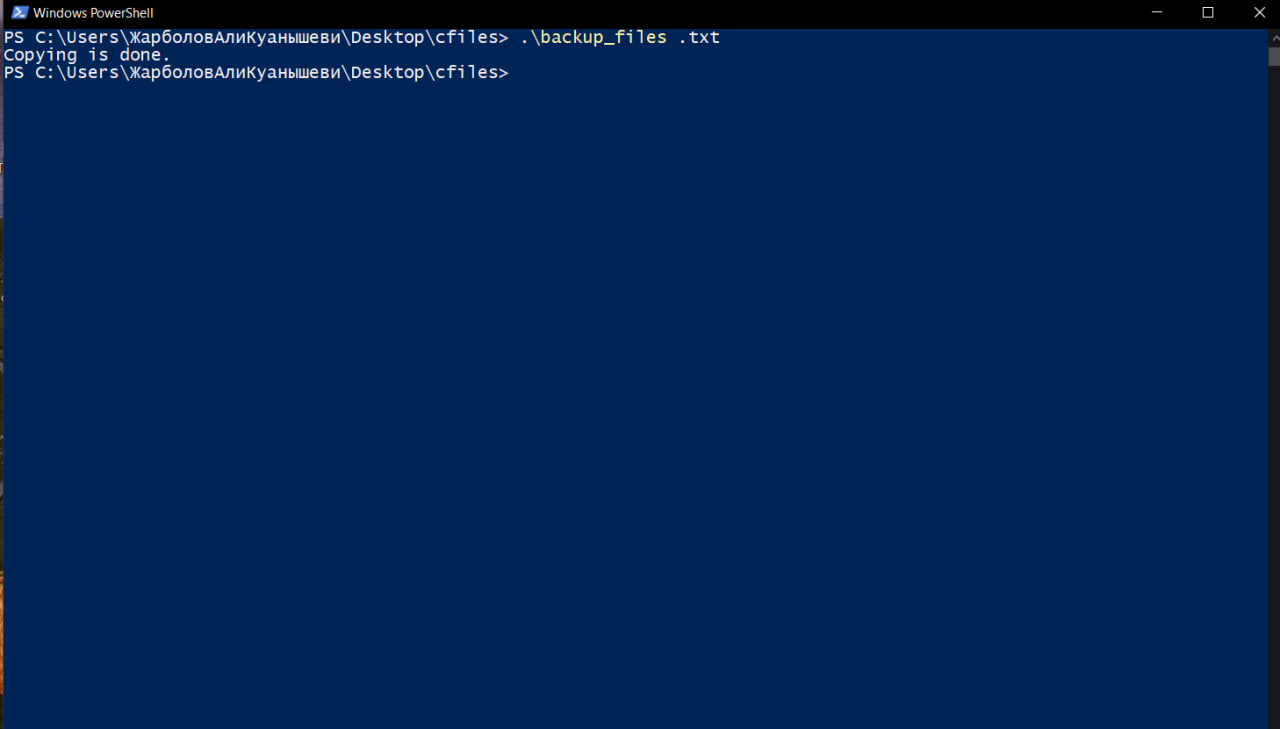
\includegraphics[width=0.5\linewidth]{Pic/lab1/photo_2025-05-21_08-15-49.jpg}
    \caption{Запуск скрипта.}
    \label{fig:RunCopy}
\end{figure}

\begin{figure}[h!]
    \centering
    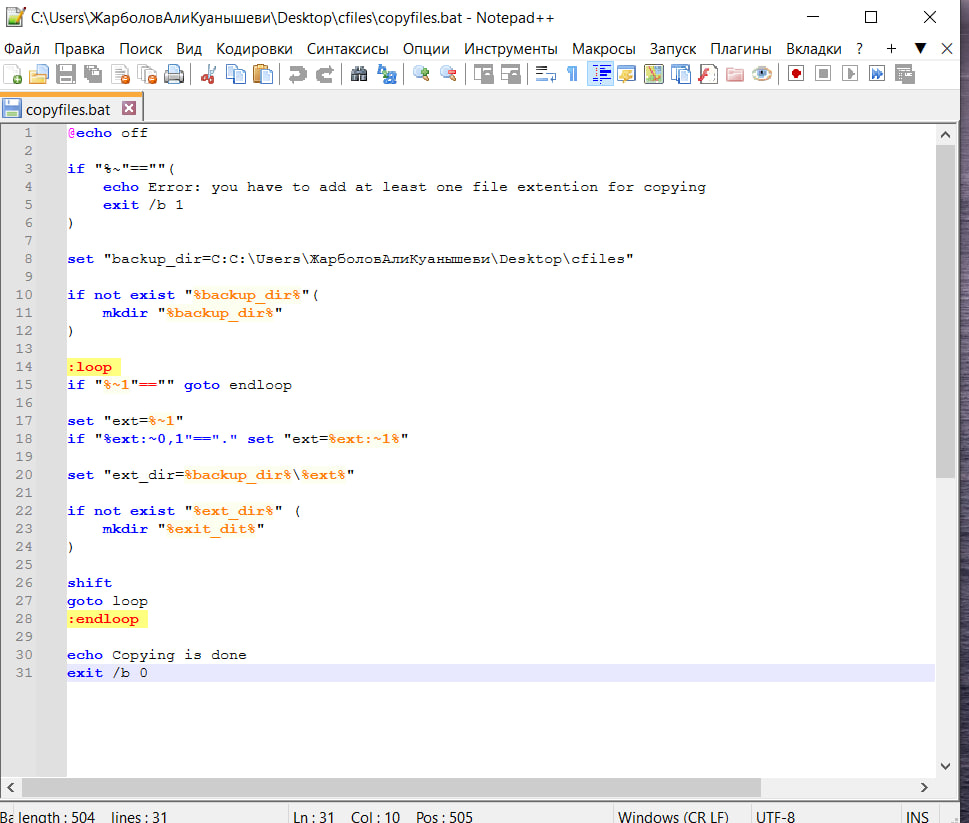
\includegraphics[width=0.9\linewidth]{Pic/lab1/photo_2025-05-21_08-15-47.jpg}
    \caption{Скрипт копирования файлов.}
    \label{fig:CopeScript}
\end{figure}

\begin{figure}[h!]
    \centering
    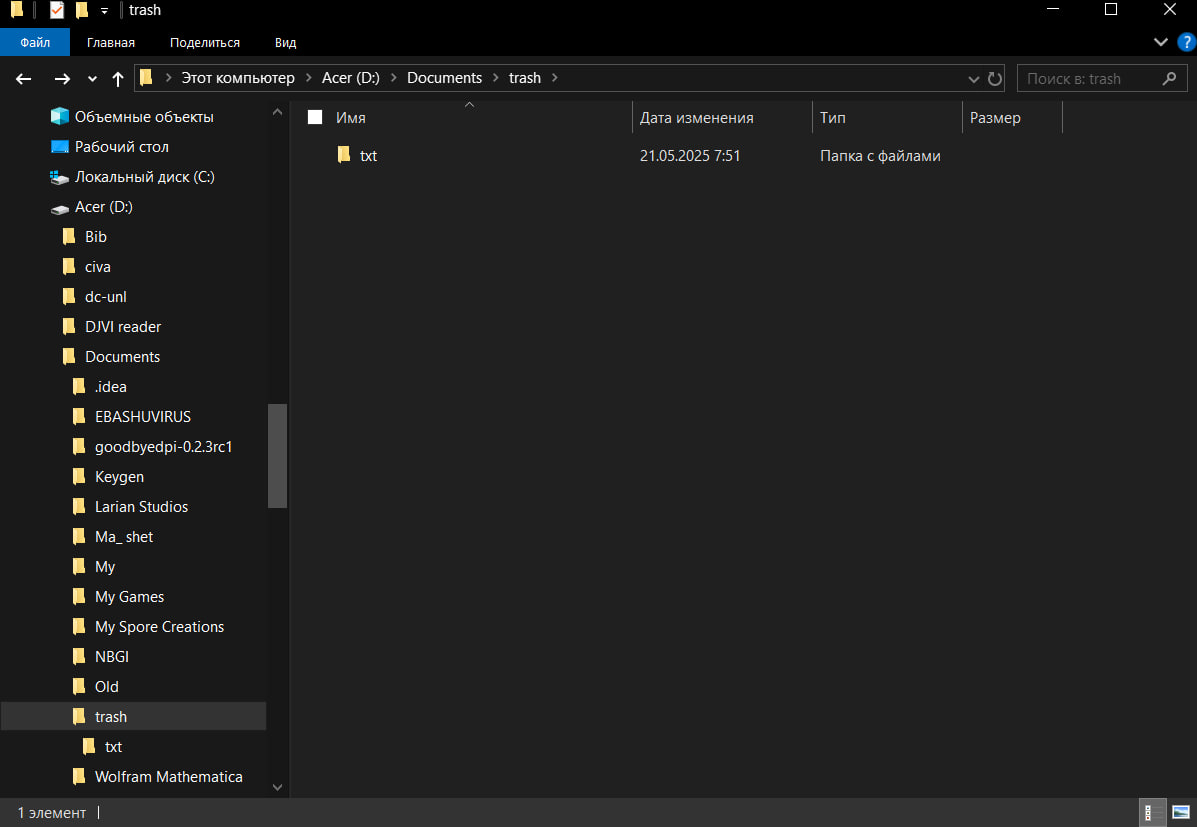
\includegraphics[width=0.5\linewidth]{Pic/lab1/photo_2025-05-21_08-15-50.jpg}
    \caption{Директория копирования.}
    \label{fig:CopyResult}
\end{figure}

Следующий скрипт, который мы напишем, будет искать файлы в указанной директории (рис. \ref{fig:FindScript}). Аналогичным образом проиходит вызов скрипта (рис. \ref{fig:FindResult}).

\begin{figure}[h!]
    \centering
    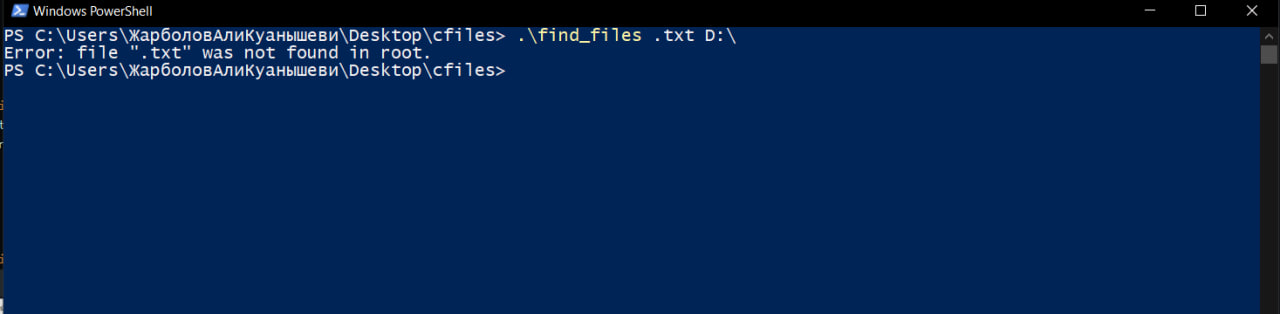
\includegraphics[width=0.5\linewidth]{Pic/lab1/photo_2025-05-21_08-15-53.jpg}
    \caption{Вызов скрипта.}
    \label{fig:FindResult}
\end{figure}

\begin{figure}[h!]
    \centering
    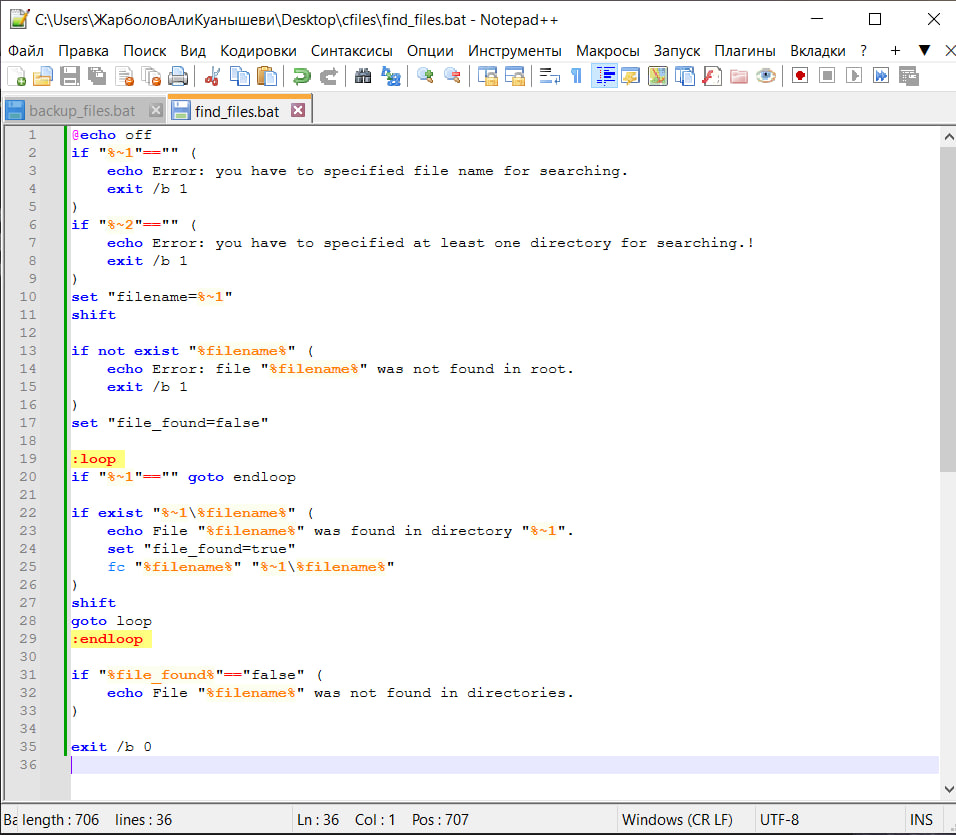
\includegraphics[width=0.9\linewidth]{Pic/lab1/photo_2025-05-21_08-15-52.jpg}
    \caption{Скрипт поиска.}
    \label{fig:FindScript}
\end{figure}

Последний скрипт, который мы напишем, это скрипт сбора информации (рис. \ref{fig:logsCreate}). Он будет собирать сведения о системе и записывать их текстовый документ. Вызываем (рис. \ref{fig:logsresult}) и видим, что логи созданы (рис. \ref{fig:logstxt}).
\begin{figure}[h!]
    \centering
    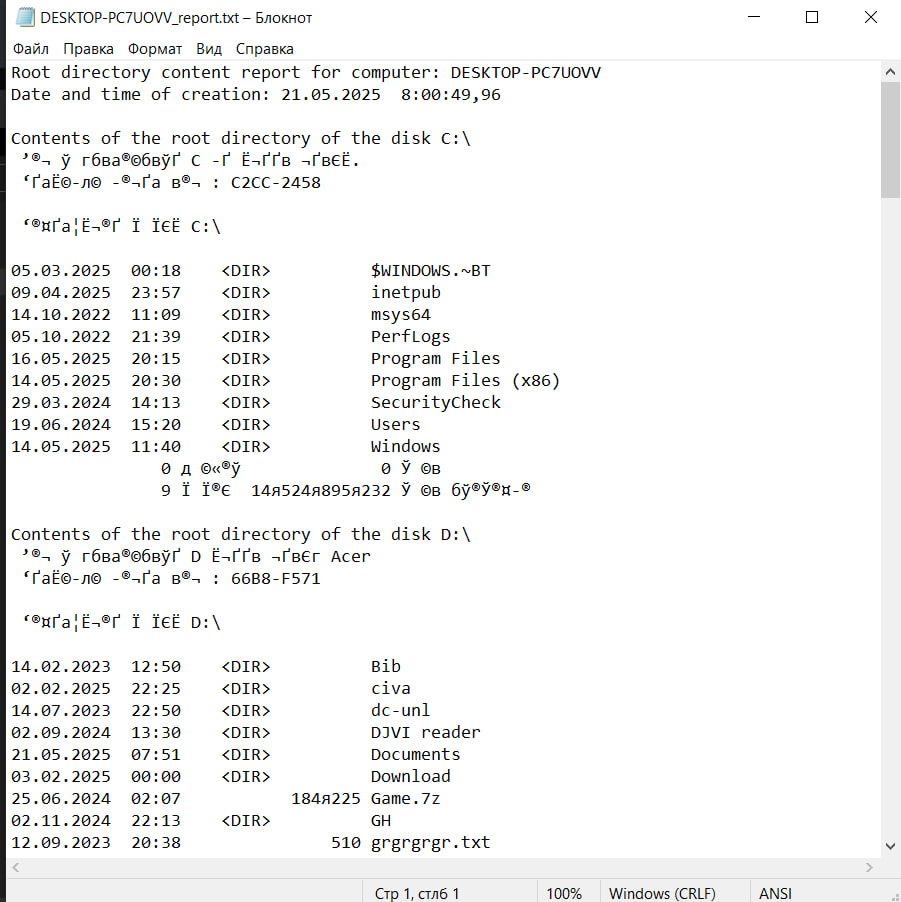
\includegraphics[width=0.3\linewidth]{Pic/lab1/photo_2025-05-21_08-15-57.jpg}
    \caption{Логи, собранные в системе.}
    \label{fig:logstxt}
\end{figure}
\begin{figure}[h!]
    \centering
    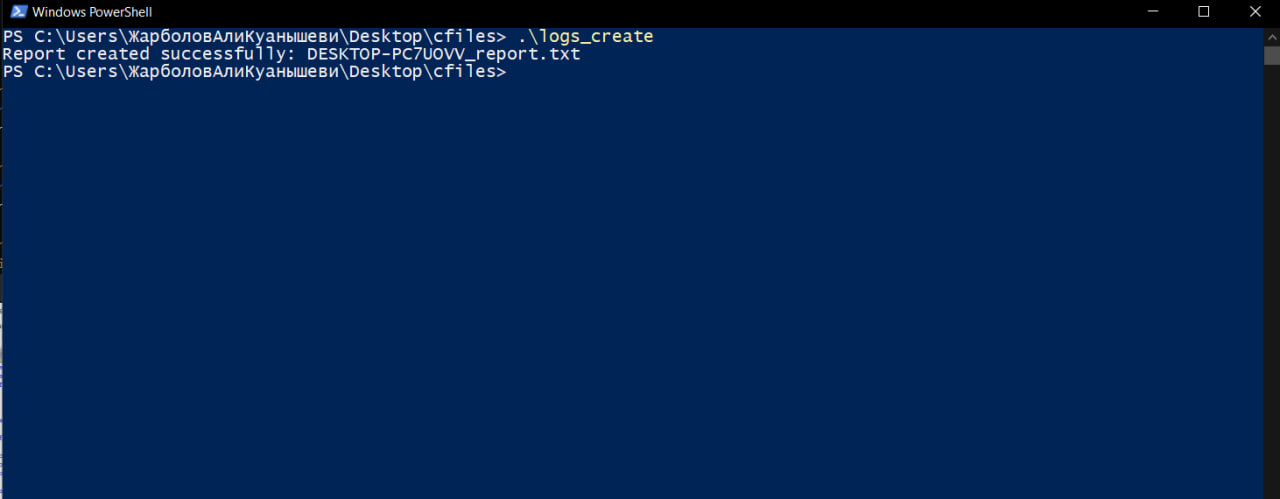
\includegraphics[width=0.5\linewidth]{Pic/lab1/photo_2025-05-21_08-15-56.jpg}
    \caption{Создание логов.}
    \label{fig:logsresult}
\end{figure}
\begin{figure}[h!]
    \centering
    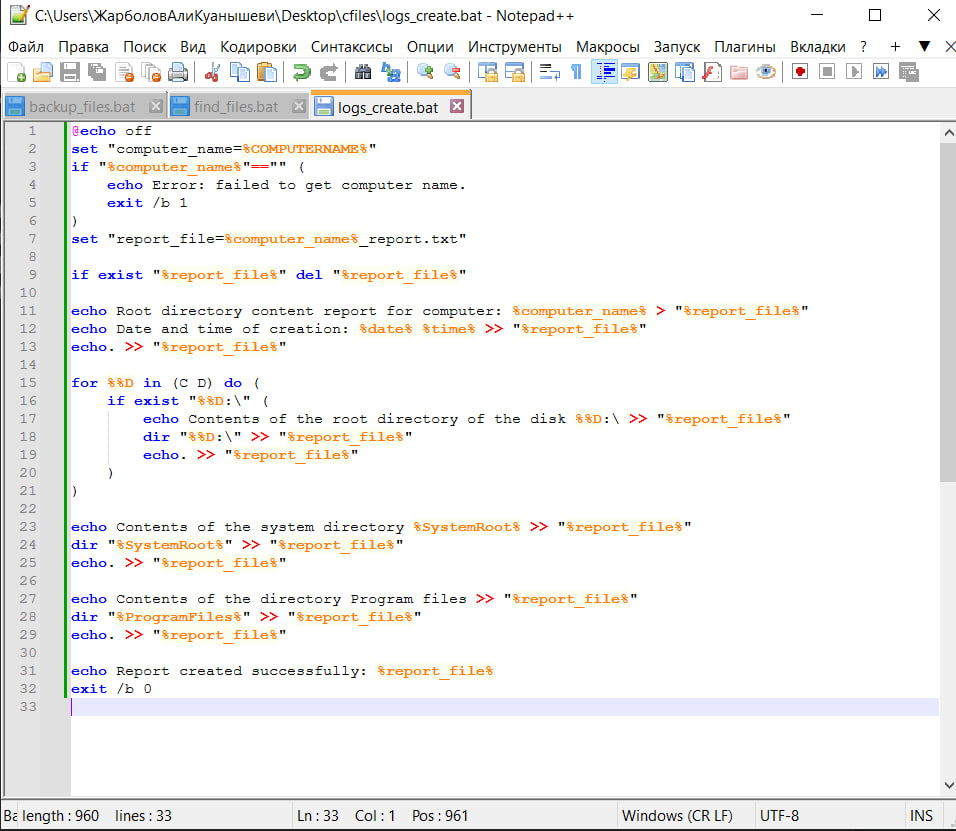
\includegraphics[width=0.6\linewidth]{Pic/lab1/photo_2025-05-21_08-15-54.jpg}
    \caption{Скрипт создания логов.}
    \label{fig:logsCreate}
\end{figure}
\begin{figure}[h!]
    \centering
    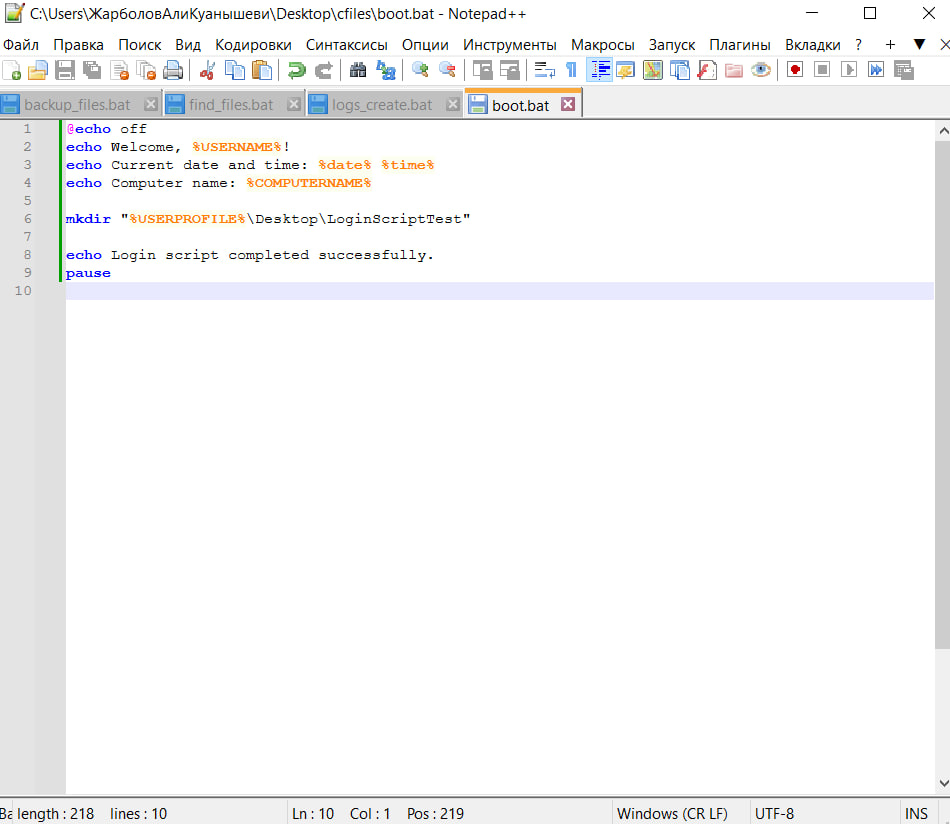
\includegraphics[width=0.6\linewidth]{Pic/lab1/photo_2025-05-21_08-16-01.jpg}
    \caption{Скрипт запуска.}
    \label{fig:boot-script}
\end{figure}

Теперь добавим скрипт запуска системы. Скрипт представлен на рисунке \ref{fig:boot-script}. Для его загрузки в систему необходимо указать в настройках пользователя сценарий входа (рис. \ref{fig:scenario}).

\begin{figure}[h!]
    \centering
    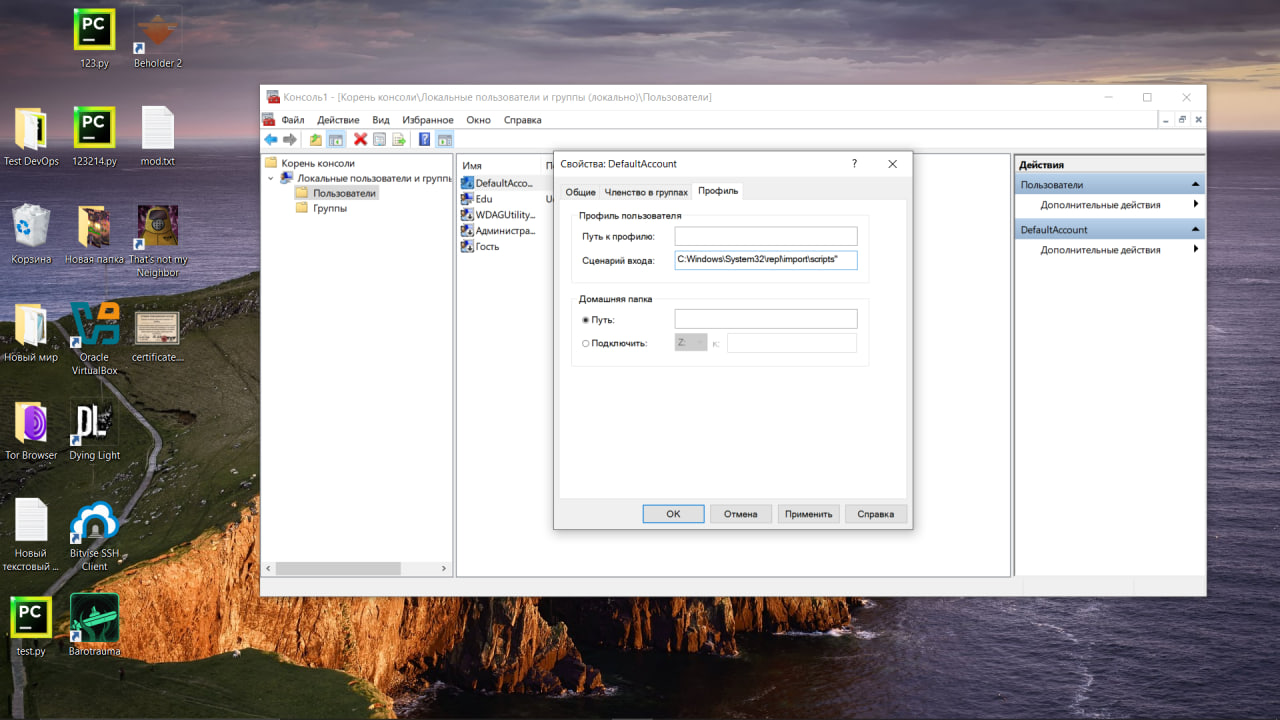
\includegraphics[width=0.4\linewidth]{Pic/lab1/photo_2025-05-21_08-15-59.jpg}
    \caption{Сценарий запуска.}
    \label{fig:scenario}
\end{figure}
\newpage
\subsection{Вывод}

В ходе данной работы мы настроили рабочую среду, учётные записи. Познакомились с командной строкой, основными командами. Также мы написали несколько скриптов исполнения командной оболочкой и сценарий запуска системы пользователем. 
\newpage


\section{Работа с файловыми системами в Windows}
В Windows используется файловая система NFTS. На этом лабораторном занятии мы разберемся с принципами её работы.
\label{LAB2}

\subsection{Цель работы}
\begin{enumerate}
    \item Изучить локальные файловые системы.
    \item Изучить способы разделения файловых ресурсов.
    \item Настроить обработку файлов с определённым расширением.
\end{enumerate}

\subsection{Ход работы}

Для того, чтобы создать папку с файловым разделом NTFS, надо зайти на системный (монтированный) диск Windows. Здесь требуется нажать правой кнопкой мыши и в контекстном меню выбрать функцию создать (рис. \ref{fig:DirEdu}). То же самое проделываем несколько раз внутри директории. Таким образом мы получим папку с вложенными файлами (рис. \ref{fig:filesinside}).
\begin{figure}[h!]
    \centering
    \begin{minipage}[p]{0.45\linewidth}
    \centering
    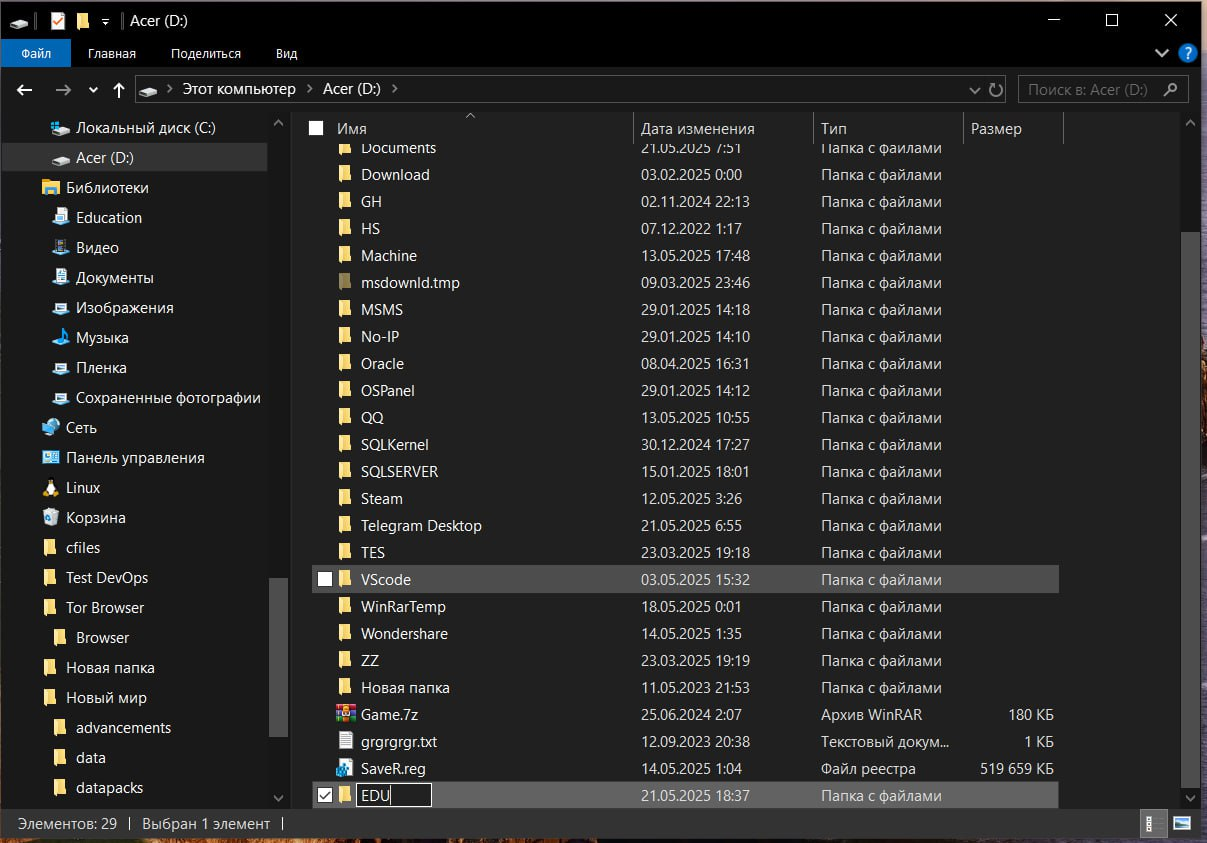
\includegraphics[width=1\linewidth]{Pic/lab2/photo_2025-05-21_21-18-26.jpg}
    \caption{Создание директории.}
    \label{fig:DirEdu}
    \end{minipage}
    \hfill
    \begin{minipage}[p]{0.45\linewidth}
    \centering
    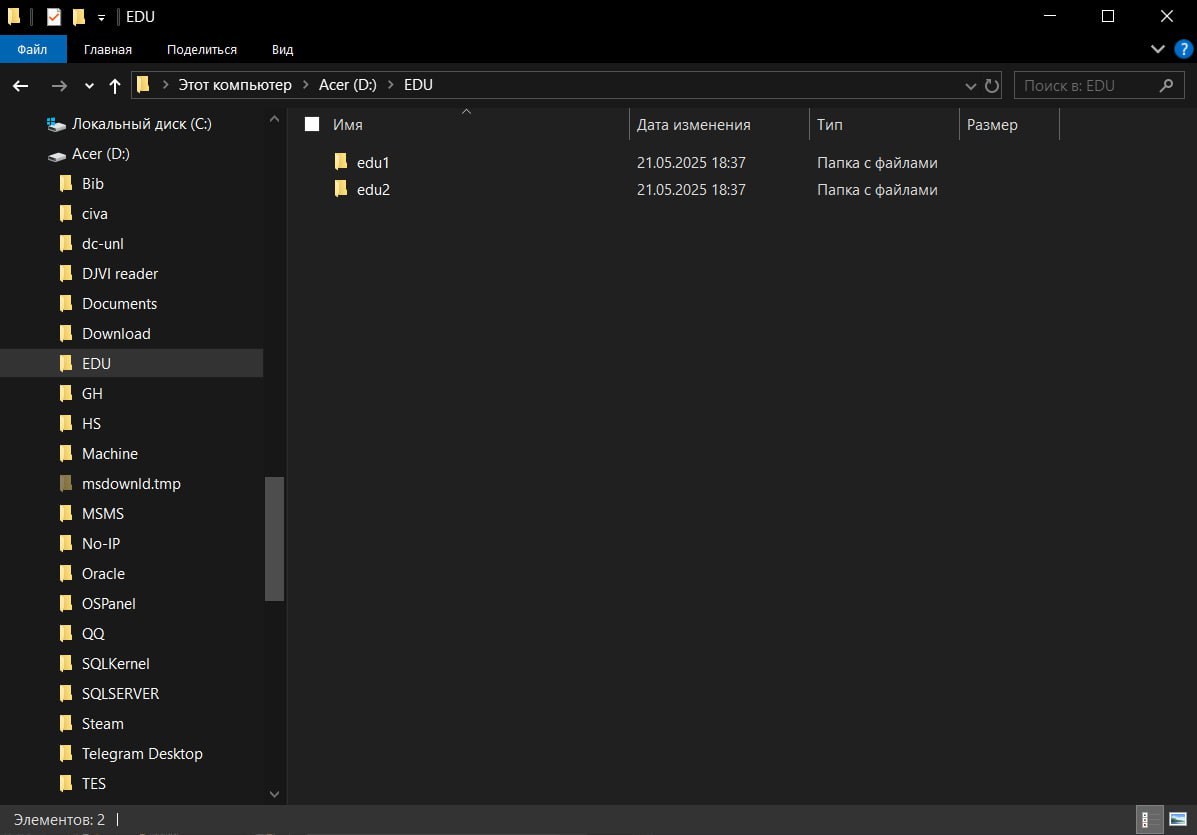
\includegraphics[width=1\linewidth]{Pic/lab2/photo_2025-05-21_21-18-28.jpg}
    \caption{Вложенные файлы.}
    \label{fig:filesinside}
    \end{minipage}
\end{figure}

\begin{figure}
\end{figure}

Настроим права доступа. Для этого кликнем правой кнопкой мыши по созданной директории, в меню выберем пункт свойства. Откроется окно, в котором есть отдельная вкладка безопасноть. Здесь мы можем увидеть всех пользователей вместе с их правами доступа. Нажав кнопку изменить, мы сможем регулирвоать права доступа пользователей (рис.\ref{fig:AccessGroups}).

По умолчанию вложенные файлы наследуют разрешения от родительской папки. Чтобы изменить права для отдельных файлов нужно изменить это в расширенных настройках.

\begin{figure}
    \centering
    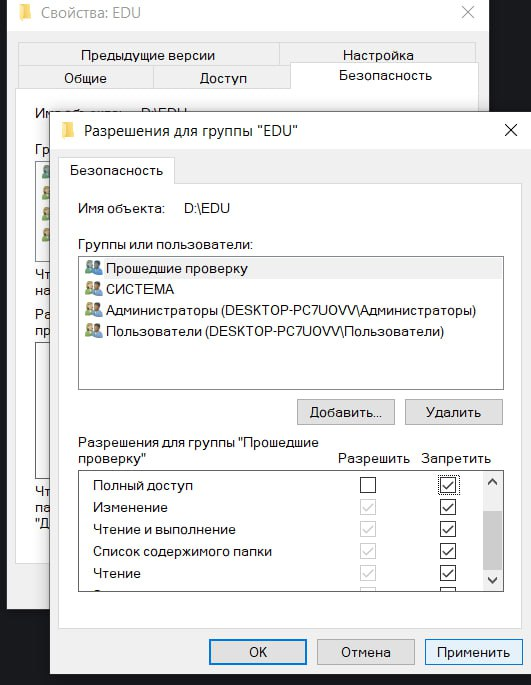
\includegraphics[width=0.5\linewidth]{Pic/lab2/photo_2025-05-21_21-18-29.jpg}
    \caption{Права доступа групп.}
    \label{fig:AccessGroups}
\end{figure}

Для любой директории можно задать специальные разрешения. Это когда пользователю выдаются особые привилегии или запреты на использование файла или папки. Чтобы выдать пользователю особые разрешения необходимо в том же меню нажать кнопку дополнительно. Откроется окно расширенных настроек, где надо нажать кнопку изменить (рис. \ref{fig:scpecialaccess}). Далее настраиваем права доступа, а также применимость этих настроек к вложенным файлам.

\begin{figure}
    \centering
    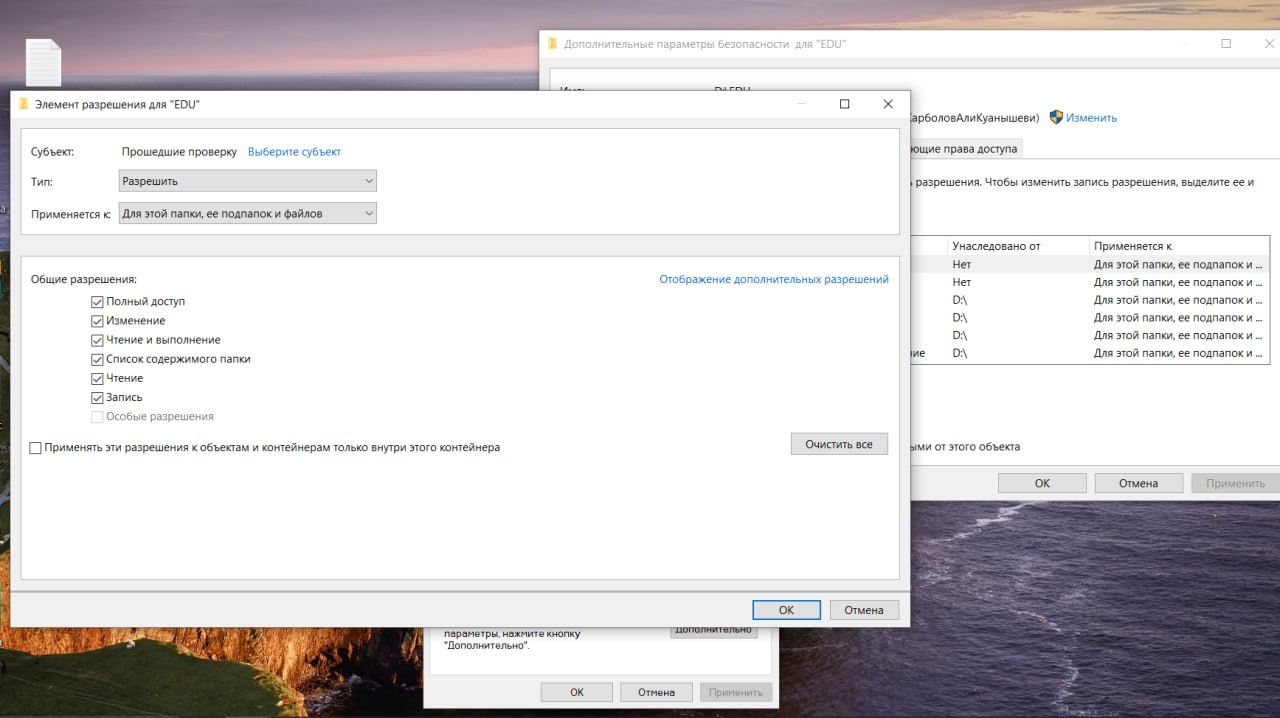
\includegraphics[width=0.8\linewidth]{Pic/lab2/photo_2025-05-21_21-18-31.jpg}
    \caption{Специальные разрешения.}
    \label{fig:scpecialaccess}
\end{figure}

В случае если некоторые разрешения назначены пользователю лично (рис. \ref{fig:AccessUsers}), а другие –
как члену группы (рис. \ref{fig:AccessEdu}), итоговые разрешения, которые получит пользователь, будут объединением этих разрешений. В случае же если пользователю налагют запрет, то он будет иметь приоритет над разрешением.

\begin{figure}[h!]
    \centering
    \begin{minipage}[p]{0.45\linewidth}
    \centering
    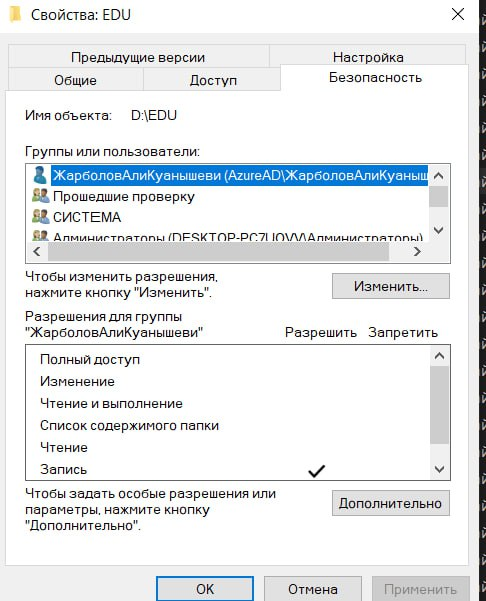
\includegraphics[width=0.5\linewidth]{Pic/lab2/photo_2025-05-21_21-18-32.jpg}
    \caption{Права доступа пользователей.}
    \label{fig:AccessUsers}
    \end{minipage}
    \hfill
    \begin{minipage}[p]{0.45\linewidth}
    \centering
    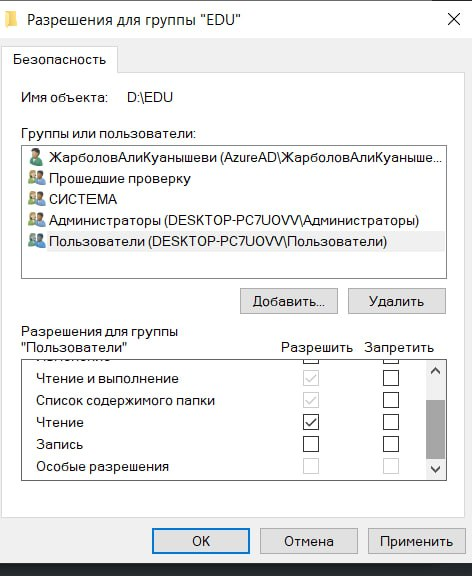
\includegraphics[width=0.5\linewidth]{Pic/lab2/photo_2025-05-21_21-18-38.jpg}
    \caption{Права доступа группы EDU.}
    \label{fig:AccessEdu}
    \end{minipage}
\end{figure}
\newpage
Как видно, пользователь может как читать содержимое директории, так и создавать новые файлы (рис. \ref{fig:AccesResult}).

\begin{figure}
    \centering
    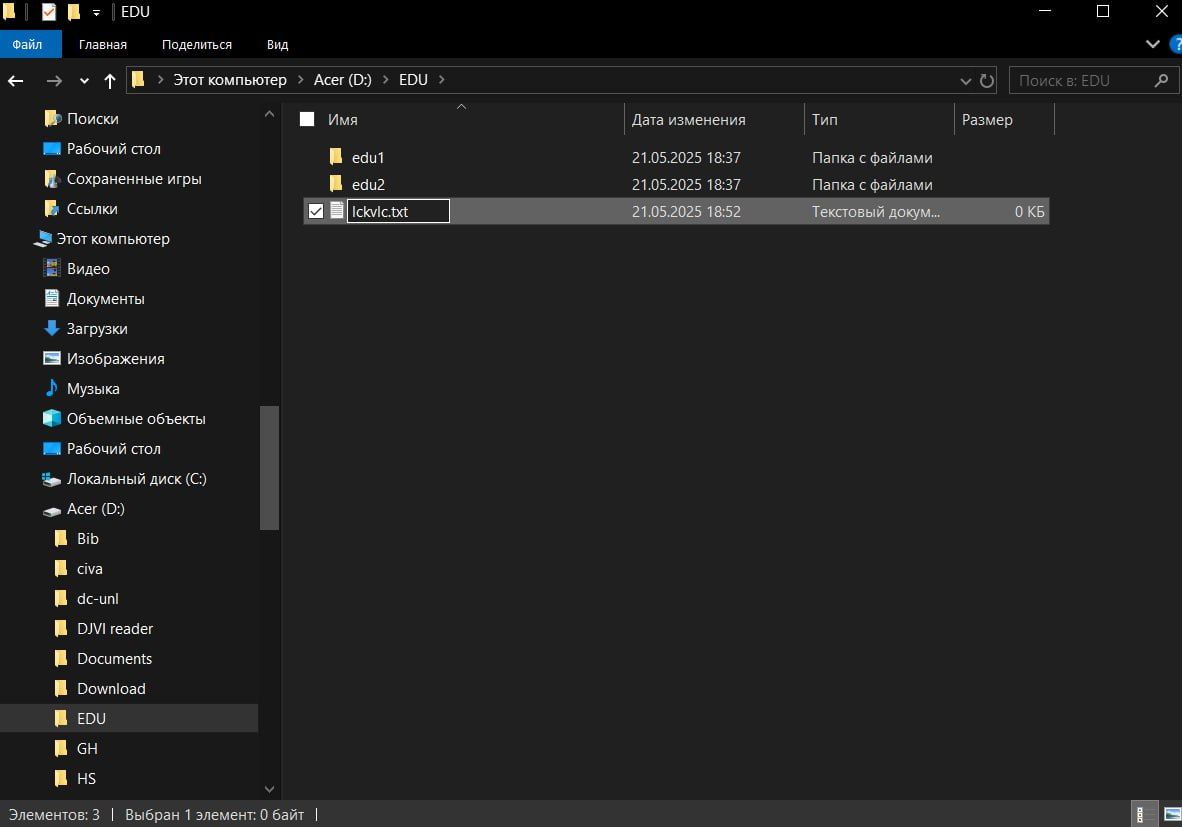
\includegraphics[width=0.5\linewidth]{Pic/lab2/photo_2025-05-21_21-18-42.jpg}
    \caption{Результирующие права пользователя.}
    \label{fig:AccesResult}
\end{figure}

В окне расширенных настроек можно не только менять права доступа, но и изменять владельца директории. При наличии достаточных полномочий, владельцем можно назначить любого пользователя. Для передачи прав над всеми вложенными файлами надо выбрать "Заменить владельца подконтейнеров и объектов".

Настраивать права доступа можно через командную оболочку Windows. Для этого используется утилита icacls. Давайте исполним следующий код:
\begin{verbatim}
        echo Some stupid content > EDU/stup.txt
        icacls EDU/stup.txt > output.txt
        type output.txt
\end{verbatim}
Команда echo создаёт поток записи в файл stup.txt, далее  при помощи icacls мы выгружаем информацию о правах доступа к файлу в другой файл - output.txt. Затем выводим на экран содержимое файла. Результат исполнения представлен на рисунке \ref{fig:icacls}.

\begin{figure}
    \centering
    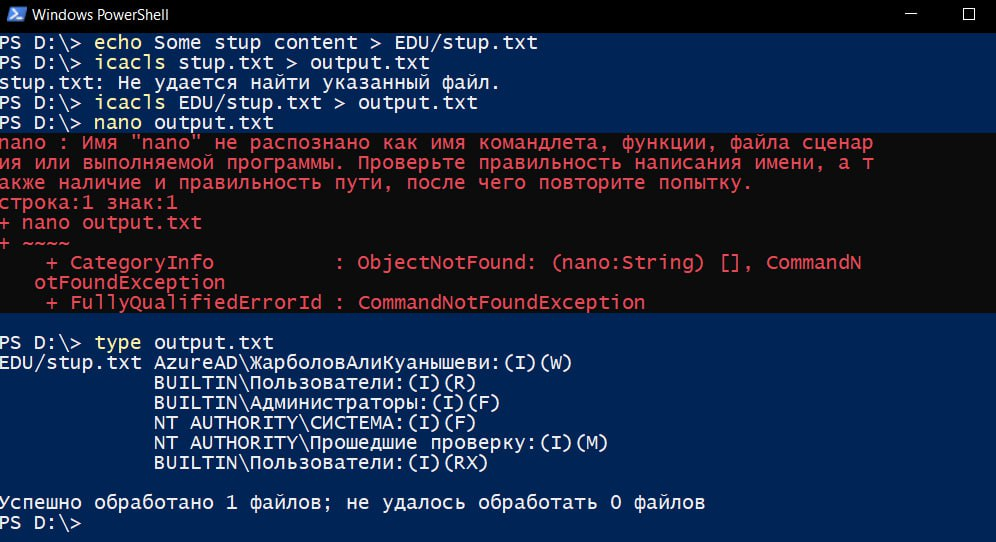
\includegraphics[width=0.5\linewidth]{Pic/lab2/photo_2025-05-21_21-18-46.jpg}
    \caption{Исполнение команд.}
    \label{fig:icacls}
\end{figure}

При помощи этой утилиты возможно изменить права доступа пользователям. Для этого мы должны использовать командную строчку в режиме администратора, иначе icacls не сможет получить доступ. Исполним следующие команды:

\begin{verbatim}
        icacls EDU /grant EDU:(R)
        icacls EDU /deny dolbaeb:(W)
\end{verbatim}

Режим (R) означает чтение, (W) - запись. Если команда написана верно, то командная оболочка отрапортует об успешном исполнении (рис. \ref{fig:icaclsAccess}). 

\begin{figure}
    \centering
    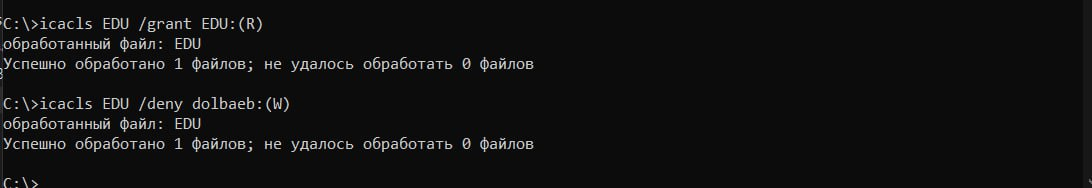
\includegraphics[width=0.5\linewidth]{Pic/lab2/photo_2025-05-21_21-18-47.jpg}
    \caption{Исполнение команд}
    \label{fig:icaclsAccess}
\end{figure}

Давайте убедимся в том, что разрешения действительно выданы (рис. \ref{fig:Edua} и \ref{fig:Dolbaeba}).

\begin{figure}[h!]
    \centering
    \begin{minipage}[p]{0.45\linewidth}
    \centering
    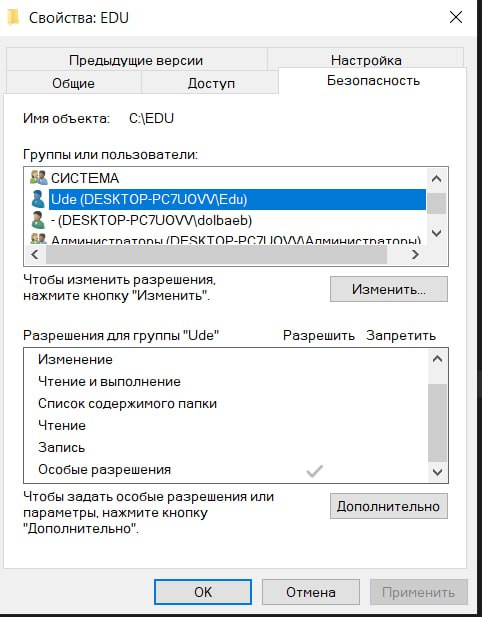
\includegraphics[width=0.5\linewidth]{Pic/lab2/photo_2025-05-21_21-18-49.jpg}
    \caption{Разрешения для группы Edu.}
    \label{fig:Edua}
    \end{minipage}
    \hfill
    \begin{minipage}[p]{0.45\linewidth}
    \centering
    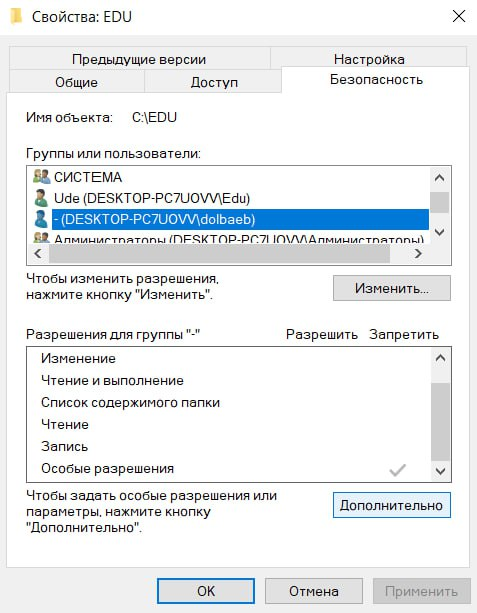
\includegraphics[width=0.5\linewidth]{Pic/lab2/photo_2025-05-21_21-18-50.jpg}
    \caption{Разрешения для пользователя.}
    \label{fig:Dolbaeba}
    \end{minipage}
\end{figure}
\newpage
Передача владения файлом/директорией уже была описана выше. Давайте проделаем эту операцию при помощи средств графисекого интерфейса (рис. \ref{fig:chown}). 

\begin{figure}[h!]
    \centering
    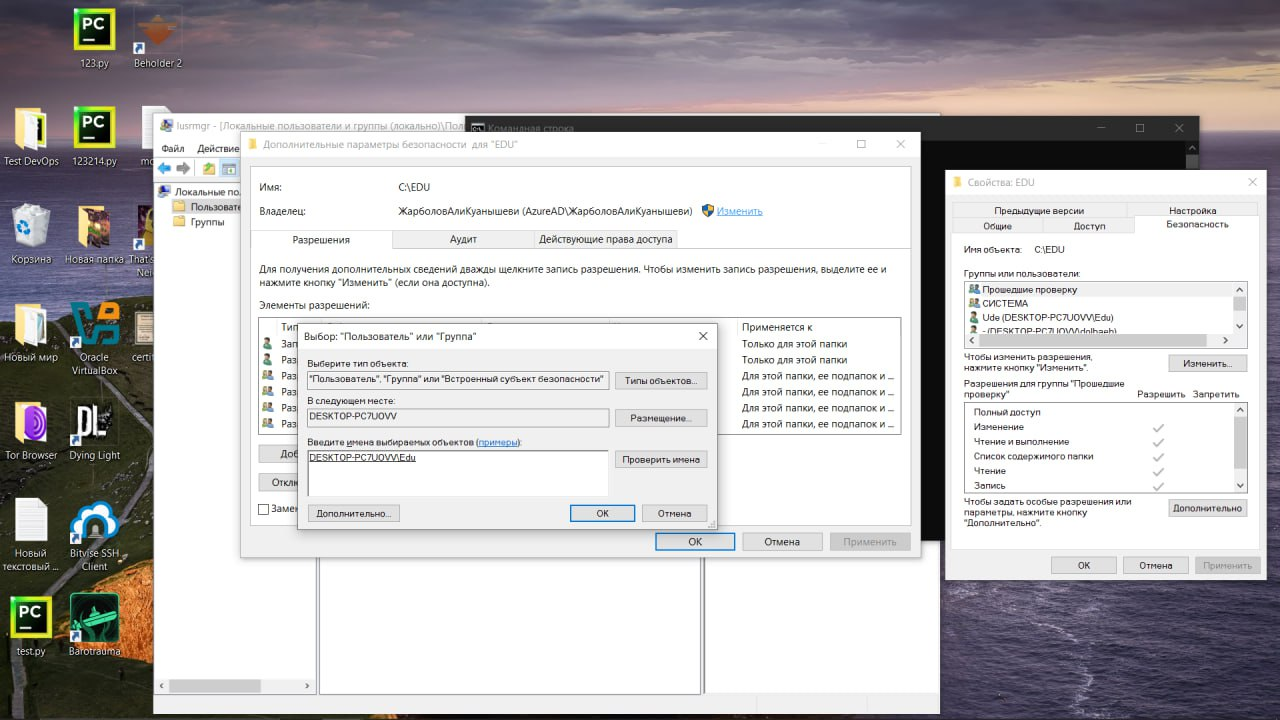
\includegraphics[width=0.5\linewidth]{Pic/lab2/photo_2025-05-21_21-18-51.jpg}
    \caption{Изменение владельца директории.}
    \label{fig:chown}
\end{figure}
То же самое можно сделать из командной строки, используя утилиту icacls и встроенную команду setowner

\begin{verbatim}
        icacls EDU /setowner Edu /r /c
\end{verbatim}

Если всё написано верно, то оболочка выдаст сообщение об успешном исполнении (рис. \ref{fig:setowner}). Сразу проверим результат исполнения (рис. \ref{fig:checkchown}). 

\begin{figure}[h!]
    \centering
    \begin{minipage}[p]{0.45\linewidth}
    \centering
    \includegraphics[width=1\linewidth]{Pic/lab2/photo_2025-05-21_21-18-53.jpg}
    \caption{Смена владельца.}
    \label{fig:setowner}
    \end{minipage}
    \hfill
    \begin{minipage}[p]{0.45\linewidth}
    \centering
    \includegraphics[width=1\linewidth]{Pic/lab2/photo_2025-05-21_21-18-54.jpg}
    \caption{Фиксируем смену владельца.}
    \label{fig:checkchown}
    \end{minipage}
\end{figure}

Для установки квоты дискового пространства необходимо открыть панель управления компьютером. Правой кнопкой мыши в программе Проводник кликаем по директории Этот компьютер. Там будет кнопка управление (рис. \ref{fig:CompControl}). Перейдите в Служебные программы, затем Управление дисками.
Правой кнопкой кликаем на нужном диске, выбираем Свойства. Там будет вкладка квота. Все действия проиллюстрированы рисунками \ref{fig:start}.
\begin{figure}[h!]
    \centering
    \includegraphics[width=0.5\linewidth]{Pic/lab2/photo_2025-05-21_21-18-56.jpg}
    \caption{Управление компьютером}
    \label{fig:CompControl}
\end{figure}

\begin{figure}[h!]
    \centering
    \includegraphics[width=0.3\linewidth]{Pic/lab2/photo_2025-05-21_21-18-57.jpg}
    \includegraphics[width=0.3\linewidth]{Pic/lab2/photo_2025-05-21_21-18-59.jpg}
    \includegraphics[width=0.3\linewidth]{Pic/lab2/photo_2025-05-21_21-19-00.jpg}
    \caption{Открытие квоты дискового пространства.}
    \label{fig:start}
\end{figure}

Нажав кнопку Ок в последнем окне, мы попадём в меню настроки квоты. Устанавливаем квоту для нашего пользователя в 2 МБ (рис. \ref{fig:quotesize}). 

\begin{figure}[h!]
    \centering
    \begin{minipage}[p]{0.45\linewidth}
    \centering
    \includegraphics[width=\linewidth]{Pic/lab2/photo_2025-05-21_21-19-02.jpg}
    \caption{Установка квоты.}
    \label{fig:quotesize}
    \end{minipage}
    \hfill
    \begin{minipage}[p]{0.45\linewidth}
    \centering
    \includegraphics[width=1\linewidth]{Pic/lab2/photo_2025-05-21_21-19-03.jpg}
    \caption{Сжатие содержимого директории.}
    \label{fig:zipdir}
    \end{minipage}
\end{figure}

Далее настроим сжатие для нашей директории. Для этого необходимо правой кнопкой мыши кликнуть по папке. В появившемся меню выбрать свойства, перейти во вкладку Общие и так окрыть дополнительные атрибуты. В этом окне надо установить галочку в пункте Сжимать содержимое для экономии места на диске (рис. \ref{fig:zipdir}). То же самое можно выполнить из командной строки командой:
\begin{verbatim}
        compact /c /s:"C:/EDU" /i /q
\end{verbatim}

Чтобы наши сжатые директории выделись в проводнике, необходимо настроить параметры Вид на верхней панели упавления. Справа будет кнопка Параметры папок. В открывшемся окне надо найти настройку Отображать сжатые или зашифрованные файлы (рис. \ref{fig:dirparam}).

\begin{figure}[h!]
    \centering
    \includegraphics[width=0.5\linewidth]{Pic/lab2/photo_2025-05-21_21-19-06.jpg}
    \caption{Параметры папок.}
    \label{fig:dirparam}
\end{figure}

В том же окне расширенных атрибутов директории можно найти настройки шифрования данных (\ref{fig:zipdir}. Установим шифрование командой. \begin{verbatim}cipher EDU\end{verbatim}

И проверим в командной строчке, что папка зашифрована (рис. \ref{fig:cipher}).

\begin{figure}
    \centering
    \includegraphics[width=0.5\linewidth]{Pic/lab2/photo_2025-05-21_21-19-09.jpg}
    \caption{Папка показана как зашифрованная.}
    \label{fig:cipher}
\end{figure}

Экспортируем сертификат. Для этого откроем утилиту certmgr.msc через win+R. Перейдём во вкладку Личное. Там будут находиться Сертификаты. Нам нужен сертификат со назначением Шифрующая файловая система. Кликаем правой кнопкой мыши, выбираем задачу Экспорт и сохраняем закрытый ключ в формате .pfx. Все шаги проиллюстрированы рисунками \ref{fig:ExportP1} и \ref{fig:ExportP2}.

\begin{figure}
    \centering
    \includegraphics[width=0.45\linewidth]{Pic/lab2/photo_2025-05-21_21-19-11.jpg}
    \includegraphics[width=0.45\linewidth]{Pic/lab2/photo_2025-05-21_21-19-12.jpg}
у    \includegraphics[width=0.45\linewidth]{Pic/lab2/photo_2025-05-21_21-19-14.jpg}
    \includegraphics[width=0.45\linewidth]{Pic/lab2/photo_2025-05-21_21-19-15.jpg}
    \caption{Экспорт сертификата.}
    \label{fig:ExportP1}
\end{figure}

\begin{figure}
    \centering
    \includegraphics[width=0.3\linewidth]{Pic/lab2/photo_2025-05-21_21-19-17.jpg}
    \includegraphics[width=0.3\linewidth]{Pic/lab2/photo_2025-05-21_21-19-19.jpg}
    \includegraphicуs[width=0.3\linewidth]{Pic/lab2/photo_2025-05-21_21-19-20.jpg}
    \caption{Экспорт сертификата.}
    \label{fig:ExportP2}
\end{figure}
\newpage

Командная строчка также предоставляет возможность создавать точки подключения и ссылки. Для этого используются встроенная утилита mklink (рис. \ref{fig:DotCon}).

\begin{figure}
    \centering
    \includegraphics[width=\linewidth]{Pic/lab2/photo_2025-05-21_21-19-21.jpg}
    \includegraphics[width=\linewidth]{Pic/lab2/photo_2025-05-21_21-19-23.jpg}
    \includegraphics[width=\linewidth]{Pic/lab2/photo_2025-05-21_21-19-24.jpg}
    \caption{Создание точек подключения и ссылок}
    \label{fig:DotCon}
\end{figure}

Проверим, можем ли смонтировать дисковое пространство в нашу систему. Нас интересует именно файловая система NTFS. Для этого мы вызовем исполнителя сочетанием win+R. Пропишем discmgmt.msc и попадем в интерфейс управления дисками. Здесь мы видим все монтированные диски. В том числе у некоторых из них указана файловая система NTFS. Что напрямую означает возможность монтирования дисков с такоим файловым разделением (рис. \ref{fig:DiskManager}).

\begin{figure}
    \centering
    \includegraphics[width=0.5\linewidth]{Pic/lab2/photo_2025-05-21_21-19-25.jpg}
    \caption{Управление дисками.}
    \label{fig:DiskManager}
\end{figure}

Теперь же проверим возможность работы с альтернативными потоками NTFS. Для этого используем команду echo, используемую во всех UX-системах. Направим поток записи в созданный нами файл. Если файл не создан, то команда echo сама его создаст (рис. \ref{fig:echo}). 

\begin{figure}[h!]
    \centering
    \includegraphics[width=\linewidth]{Pic/lab2/photo_2025-05-21_21-19-27.jpg}
    \caption{Поток записи echo.}
    \label{fig:echo}
\end{figure}

Попробуем использовать несколько потоков. Для этого одному из них выдадим метку :hidden. Используя метки потоков, мы можем выводить разные результаты (рис. \ref{fig:hiddenecho}). 

\begin{figure}
    \centering
    \includegraphics[width=\linewidth]{Pic/lab2/photo_2025-05-21_21-19-28.jpg}
    \caption{Помеченный поток записи.}
    \label{fig:hiddenecho}
\end{figure}
\newpage
Теперь следуя инструкции с рисунка \ref{fig:AccessUsers}, ограничим себе доступ к директории EDU. Как видно на рисунке \ref{fig:DeniedAccess}, мы не можем войти в папку. 
\begin{figure}[h!]
    \centering
    \includegraphics[width=0.5\linewidth]{Pic/lab2/photo_2025-05-21_21-19-31.jpg}
    \caption{Отказ в доступе.}
    \label{fig:DeniedAccess}
\end{figure}

Следуя инструкциям с рисунка \ref{fig:scpecialaccess}, открываем расширенные настройки доступа. Там есть отдельная вкладка аудита, в которой мы можем подключить кнопкой добавить сбор логов действий пользователей в определённых директориях (рис. \ref{fig:audit}). 

\begin{figure}[h!]
    \centering
    \includegraphics[width=0.5\linewidth]{Pic/lab2/photo_2025-05-21_21-19-32.jpg}
    \caption{Подключение аудита}
    \label{fig:audit}
\end{figure}

Через исполнителя (win+R) открываем утилиту eventvwr.msc. Это менеджер событий, который собирает информацию обо всех службах, процессах системы. Здесь выберем вкладку безопасность и увидим, что жунал аудита сообщает нам о попытках входа в директорию (рис. \ref{fig:EventManager}).

\begin{figure}[h!]
    \centering
    \includegraphics[width=0.5\linewidth]{Pic/lab2/photo_2025-05-21_21-19-33.jpg}
    \caption{Журнал аудита.}
    \label{fig:EventManager}
\end{figure}

Также выполним проверку фрагментации дискового пространства. Для этого исполним команду с рисунка \ref{fig:discfrag}.

\begin{figure}[h!]
    \centering
    \includegraphics[width=0.9\linewidth]{Pic/lab2/photo_2025-05-21_21-19-34.jpg}
    \caption{Фрагментация диска}
    \label{fig:discfrag}
\end{figure}

Перейдем к настройке сетевого интерфейса и параметров общего файлового пространства. Для начала выясним домен, к которому принадлежит компьютер. Для этого в командной оболочке вводим команду hostname утилиты nslookup (рис. \ref{fig:hostname}).
 
\begin{figure}[h!]
    \centering
    \includegraphics[width=\linewidth]{Pic/lab2/photo_2025-05-21_21-19-36.jpg}
    \caption{Команда hostname.}
    \label{fig:hostname}
\end{figure}
\newpage
Далее по инструкции из главы \ref{GL1} добавим оснастку Общие папки (рис. \ref{fig:CommonFiles}).

\begin{figure}
    \centering
    \includegraphics[width=0.5\linewidth]{Pic/lab2/photo_2025-05-22_00-25-53.jpg}
    \caption{Оснастка Общие папки.}
    \label{fig:CommonFiles}
\end{figure}

Выполняем настройку как на рисунках \ref{fig:CFprop}:

\begin{figure}[h!]
    \centering
    \includegraphics[width=0.5\linewidth]{Pic/lab2/photo_2025-05-22_00-25-55.jpg}
    \includegraphics[width=0.5\linewidth]{Pic/lab2/photo_2025-05-22_00-25-57.jpg}
    \includegraphics[width=0.5\linewidth]{Pic/lab2/photo_2025-05-22_00-25-58.jpg}
    \caption{Настройка оснастки.}
    \label{fig:CFprop}
\end{figure}

Когда мы добавили оснастку, то через командную строку выполним создание общих папок как общедоступных, так и скрытых (рис. \ref{fig:HiddenShare}). Важно совершать эти операции от имени администратора, т. к. иначе пользователь может не иметь достаточных полномочий.

\begin{figure}
    \centering
    \includegraphics[width=0.5\linewidth]{Pic/lab2/photo_2025-05-22_00-26-00.jpg}
    \caption{Создание директорий общего пользования}
    \label{fig:HiddenShare}
\end{figure}

Установим разрешений доступа. Для этого мы используем инструкции с рисунка \ref{fig:AccessGroups} для локальных разрешений (NTFS). Для настроек общего доступа перейдём во вкладку Доступ. Откроем расширенную настройку и внесём пользователей, которым будет открыт доступ (рис. \ref{fig:NetAccess}).

\begin{figure}[h!]
    \centering
    \includegraphics[width=0.5\linewidth]{Pic/lab2/photo_2025-05-22_00-26-01.jpg}
    \caption{Доступ к сети}
    \label{fig:NetAccess}
\end{figure}

При доступе по сети применяются оба вида разрешений. Результирующие права - наиболее ограничивающие из двух наборов. Поэтому важно настроить оба эих вида разрешений, ведь даже при наличии сетевого доступа, пользователь может не открыть папку общего пользователя из-за локальных ограничений. Настроим локальных доступ (рис. \ref{fig:localacces}).

\begin{figure}[h!]
    \centering
    \includegraphics[width=0.5\linewidth]{Pic/lab2/photo_2025-05-22_00-26-03.jpg}
    \caption{Локальные разрешения.}
    \label{fig:localacces}
\end{figure}

\begin{figure}[h!]
    \centering
    \includegraphics[width=0.5\linewidth]{Pic/lab2/photo_2025-05-22_00-26-05.jpg}
    \caption{Проверим подключение.}
    \label{fig:checkcon}
\end{figure}
\newpage
Установим возможность работы с файлами в автономном режиме. Для этого в свойствах открываем вкладку Общий доступ. Нажмаем Кэширование. И выбираем один из вариантов:
\begin{enumerate}
    \item Только файлы и программы, которые используются пользователем, автоматически будут доступны автономно
    \item Все файлы и программы, открытые пользователями из общей папки, автоматически будут доступны автономно
    \item Файлы и программы из общей папки недоступны автономно
\end{enumerate}

Если вы подключите автономный доступ к файлам, важно знать, что синхронизация происходит по одному из четырёх вариантов:
\begin{enumerate}
    \item Автоматическая синхронизация - при подключении к сети.
    \item Ручная синхронизация: через проводник, либо Центр синхронизации.
    \item По расписанию: через Центр синхронизации доступна настройка нового расписания синхронизации.
    \item Принудительная синхронизация через командную строку.
\end{enumerate}

В довершении лабораторной работы создадим своё собственное расширение для системы Windows и внесём его в системный регистр. Снача сочетанием клавиш win+R исполняем запуск regedit. Откроется интерфейс редактора реестра. Выбираем раздел HKEY\_CLASSES\_ROOT. В нём необходимо создать новый раздел (рис. \ref{fig:new_r}).

\begin{figure}[h!]
    \centering
    \includegraphics[width=0.5\linewidth]{Pic/lab2/photo_2025-05-22_00-26-11.jpg}
    \caption{ПКМ+создать новый раздел.}
    \label{fig:new_r}
\end{figure}

\begin{figure}[h!]
    \centering
    \includegraphics[width=0.5\linewidth]{Pic/lab2/photo_2025-05-22_00-26-13.jpg}
    \caption{Задаём уникальное название.}
    \label{fig:NewRComplete}
\end{figure}

Внутри раздела необходимо создать файловую систему (рис. \ref{fig:extenddir}). Создаём директорию Shell. Эта директория считается директорией командной оболочки, именно здесь находятся команды, исполняемые оболочкой Windows. Далее создаём два сценария: open, print. Внутри них необходимо создать папки command, в которых мы опишем команды, исполняемые терминалом. Напишем всего две команды: 
\begin{verbatim}
        notepad.exe "%1"
        :: Первая команда
        more < "%1"
        :: Вторая команда
\end{verbatim}

\begin{figure}[h!]
    \centering
    \includegraphics[width=\linewidth]{Pic/lab2/photo_2025-05-22_00-26-14.jpg}
    \caption{Файловая система расширения.}
    \label{fig:extenddir}
\end{figure}

Теперь для файла с нашим расширением двойной щелчок откроет файл в блокноте. Печать создаст поток чтения в консоль. Добавим команды Зашифровать/Дешифровать в контекстное меню. Перейдём в реестре в директорию:
\begin{verbatim}
HKEY_LOCAL_MACHINE\SOFTWARE\Microsoft\Windows\CurrentVersion\Explorer\Advanced
\end{verbatim}

Создадим раздел DWORD (32 бита) EncryptionContext Menu (рис. \ref{fig:contextmenu}) и зададим значение 1.

\begin{figure}[h!]
    \centering
    \includegraphics[width=0.5\linewidth]{Pic/lab2/photo_2025-05-22_00-26-20.jpg}
    \caption{Создание раздела контекстного меню.}
    \label{fig:contextmenu}
\end{figure}
\newpage
Для применения изменений перезапустим систему. В реестре также находятся два раздела
\begin{verbatim}
HKEY_LOCAL_MACHINE\SOFTWARE\Microsoft\Windows\CurrentVersion\Run
HKEY_LOCAL_MACHINE\SOFTWARE\Microsoft\Windows\CurrentVersion\RunOnce
\end{verbatim}

Run - программы, запускаемые при входе каждого пользователя. RunOnce - программы, которые выполняются один раз при следующем входе. Каждый параметр представляет собой программу для автозагрузки. Значение параметра - путь к исполняемому файлу

Создадим файл расширения .reg. Изменим немного исполняемые команды и импортируем обратьно в регистр (рис. \ref{fig:REG}). 

\begin{figure}[h!]
    \centering
    \includegraphics[width=0.3\linewidth]{Pic/lab2/photo_2025-05-22_00-26-22.jpg}
    \caption{REG-файл, который монтирует наше расширение.}
    \label{fig:REG}
\end{figure}

Дважды кликнем и внесём изменения в регистр.

\begin{figure}[h!]
    \centering
    \includegraphics[width=0.5\linewidth]{Pic/lab2/photo_2025-05-22_00-26-24.jpg}
    \caption{Внесение изменений в регистр}
    \label{fig:REGChange}
\end{figure}

\begin{figure}[h!]
    \centering
    \includegraphics[width=0.5\linewidth]{Pic/lab2/photo_2025-05-22_00-26-29.jpg}
    \caption{Исполнение файла.}
    \label{fig:new_extend}
\end{figure}

\subsection{Вывод}

В ходе выполнения лабораторной работы мы изучили файловую систему Windows, способы разделения файловых ресурсов и настроили обработку файлов определённого расширения. В целом, мы поняли, что Windows не предназначения для многопользовательского доступа. Инстументы работы примитивны. 

Система расширений, настраиваемая через регистры, совершенно бесполезна, ведь, даже настроив расширения для всевозможных файлов, мы всё равно можем замаскивароть .bat файл под png, задав нужное расширение. 

Windows удобна в первую очередь для личного пользования. Для разработки системы Linux подходят куда лучше. 

\newpage
\section{Разграничение доступа к объектам файловой системы}
В таблицы из баз данных можно загружать данные из источника. Для этого существуют специальные команды transact.
\label{LAB3}
\subsection{Цель работы}
\begin{itemize}
    \item Изучить T-SQL команды INSERT, INSERT-SELECT.
    \item Внести данные из файла в базу данных.
    \item Добавить запросы данных из таблиц.
    \item Добавить с таблицы данные о книге Карпова Т. С. Базы данных: модели, разработка, реализация, 2001.
\end{itemize}
\subsection{Ход работы}

\subsection{Вывод}
В ходе выполнения данной лабораторной работы мы изучили команды INSERT, SELECT. Внесли данные из файла в базу данных. Написали запросы данных из таблиц и выполнили дополнительное задание. 

\section{Виртуальная машина Linux}
В этой лабораторной работе мы развернём виртуальную машину с системой Linux, используя программу Oracle VirtualBox. 

\subsection{Цель работы}
\begin{itemize}
    \item Установить Oracle VirtualBox.
    \item Установить Debian.
\end{itemize}
\subsection{Ход работы}

Первым делом необходимо установить Oracle VirtualBox. Для это надо перейти на \href{https://www.virtualbox.org/}{официальный сайт}. Установка виртуальной машины проходит в штатном режиме. Важно лишь не использовать кириллические символы в пути до места установки.

Когда мы установим VirtualBox, необходимо настроить программу. Далее перечислены рисунки с нужными настройками.

\begin{figure}[h!]
    \centering
    \includegraphics[width=0.5\linewidth]{Pic/lab4/Вставленное изображение.png}
    \caption{Создаём новую вируатльную машину.}
    \label{fig:enter-label}
\end{figure}

\begin{figure}[h!]
    \centering
    \includegraphics[width=0.3\linewidth]{Pic/lab4/Вставленное изображение (2).png}
    \caption{Называем машину и выбираем расположение.}
    \label{fig:enter-label}
\end{figure}

\begin{figure}[h!]
    \centering
    \includegraphics[width=0.3\linewidth]{Pic/lab4/Вставленное изображение (3).png}
    \caption{Выделаем системные ресурсы.}
    \label{fig:enter-label}
\end{figure}

\begin{figure}[h!]
    \centering
    \includegraphics[width=0.3\linewidth]{Pic/lab4/Вставленное изображение (4).png}
    \caption{Выделяем дисковое пространство.}
    \label{fig:enter-label}
\end{figure}

\begin{figure}[h!]
    \centering
    \includegraphics[width=0.3\linewidth]{Pic/lab4/Вставленное изображение (5).png}
    \caption{Ждём загрузки.}
    \label{fig:enter-label}
\end{figure}

\begin{figure}[h!]
    \centering
    \includegraphics[width=0.3\linewidth]{Pic/lab4/Вставленное изображение (6).png}
    \caption{Виртуальная машина инсталирована.}
    \label{fig:installedVB}
\end{figure}
\newpage
Виртуальная машина готова(рис. \ref{fig:installedVB}). В данный момент она не имеет операционной системы. Мы можем попробовать её включить, но дальше grab rescue зайти не сможем. Прежде надо произвести настройку самой машины. Для этого надо зайти в настройки виртуальной машины, включить экспертный режим.

\begin{figure}[h!]
    \centering
    \includegraphics[width=0.3\linewidth]{Pic/lab4/Вставленное изображение (7).png}
    \caption{Устанавливаем место для точек восстановления.}
    \label{fig:enter-label}
\end{figure}

\begin{figure}[h!]
    \centering
    \includegraphics[width=0.3\linewidth]{(8)}
    \caption{Выбираем монтируемый образ.}
    \label{fig:enter-label}
\end{figure}

\begin{figure}[h!]
    \centering
    \includegraphics[width=0.3\linewidth]{Pic/lab4/Вставленное изображение (9).png}
    \caption{Будем использовать 11 версию Debian.}
    \label{fig:enter-label}
\end{figure}
\newpage
Посл того, как мы монтировали образ в виртуальную машину, необходимо загрузить её. При запуске у нас откроется программа установки Debian 11. Действуем по инструкциям.

\begin{figure}[h!]
    \centering
    \includegraphics[width=0.3\linewidth]{Pic/lab4/Вставленное изображение (12).png}
    \caption{Выбираем обычную установку.}
    \label{fig:enter-label}
\end{figure}

\begin{figure}[h!]
    \centering
    \includegraphics[width=0.3\linewidth]{Pic/lab4/Вставленное изображение (13).png}
    \caption{Желательно выбрать язык английский, так как это гарантирует читаемость текста.}
    \label{fig:enter-label}
\end{figure}

\begin{figure}[h!]
    \centering
    \includegraphics[width=0.3\linewidth]{Pic/lab4/Вставленное изображение (14).png}
    \caption{Выбираем регион правильно. Это влияет на работу сервера и предлагаемые репозитории пакетов.}
    \label{fig:enter-label}
\end{figure}

\begin{figure}[h!]
    \centering
    \includegraphics[width=0.3\linewidth]{Pic/lab4/Вставленное изображение (15).png}
    \includegraphics[width=0.3\linewidth]{Pic/lab4/Вставленное изображение (16).png}
    \caption{Регион выбираем Европа, Российская федерация.}
    \label{fig:enter-label}
\end{figure}

\begin{figure}[h!]
    \centering
    \includegraphics[width=0.3\linewidth]{Pic/lab4/Вставленное изображение (17).png}
    \includegraphics[width=0.3\linewidth]{Pic/lab4/Вставленное изображение (18).png}
    \caption{Устанавливаем язык по умолчанию en\_US UTF-8. Это ппредовратит проблемы в будущем.}
    \label{fig:enter-label}
\end{figure}

\begin{figure}[h!]
    \centering
    \includegraphics[width=0.4\linewidth]{Pic/lab4/Вставленное изображение (18).png}
    \caption{Дожидаемся установки}
    \label{fig:enter-label}
\end{figure}

\begin{figure}[h!]
    \centering
    \includegraphics[width=0.4\linewidth]{Pic/lab4/Вставленное изображение (19).png}
    \caption{Устанавливаем язык по умолчанию en\_US UTF-8. Это ппредовратит проблемы в будущем.}
    \label{fig:enter-label}
\end{figure}

\begin{figure}[h!]
    \centering
    \includegraphics[width=0.4\linewidth]{Pic/lab4/Вставленное изображение (21).png}
    \caption{Вводим имя хоста.}
    \label{fig:enter-label}
\end{figure}
\newpage
\begin{figure}[h!]
    \centering
    \includegraphics[width=0.3\linewidth]{Pic/lab4/Вставленное изображение (22).png}
    \caption{Устанавливаем пароль для рут-пользователя}
    \label{fig:enter-label}
\end{figure}

\begin{figure}[h!]
    \centering
    \includegraphics[width=0.3\linewidth]{Pic/lab4/Вставленное изображение (23).png}
    \includegraphics[width=0.3\linewidth]{Pic/lab4/Вставленное изображение (24).png}
    \caption{Заполняем данные обычного пользователя}
    \label{fig:enter-labe}
\end{figure}

\begin{figure}[h!]
    \centering
    \includegraphics[width=0.3\linewidth]{Pic/lab4/Вставленное изображение (25).png}
    \caption{Вводим пароль пользователя}
    \label{fig:enter-label}
\end{figure}

\begin{figure}[h!]
    \centering
    \includegraphics[width=0.3\linewidth]{Pic/lab4/Вставленное изображение (26).png}
    \caption{Устанавливаем системное время}
    \label{fig:enter-label}
\end{figure}

\begin{figure}[h!]
    \centering
    \includegraphics[width=0.3\linewidth]{Pic/lab4/Вставленное изображение (27).png}
    \caption{Выбираем просто монтирование диска.}
    \label{fig:enter-label}
\end{figure}

\begin{figure}[h!]
    \centering
    \includegraphics[width=0.3\linewidth]{Pic/lab4/Вставленное изображение (28).png}
    \caption{Выбираем место установки.}
    \label{fig:enter-label}
\end{figure}

\begin{figure}[h!]
    \centering
    \includegraphics[width=0.3\linewidth]{Pic/lab4/Вставленное изображение (29).png}
    \caption{Выбираем установку в единый корень}
    \label{fig:enter-label}
\end{figure}


\begin{figure}[h!]
    \centering
    \includegraphics[width=0.3\linewidth]{Pic/lab4/Вставленное изображение (31).png}
    \caption{Соглашаемся}
    \label{fig:enter-label}
\end{figure}

\begin{figure}[h!]
    \centering
    \includegraphics[width=0.3\linewidth]{Pic/lab4/Вставленное изображение (32).png}
    \caption{Ждём установки}
    \label{fig:enter-label}
\end{figure}

\begin{figure}[h!]
    \centering
    \includegraphics[width=0.3\linewidth]{Pic/lab4/Вставленное изображение (34).png}
    \caption{Выбираем, к какому серверу будем подключаться при обращениях в репозиторий.}
    \label{fig:enter-label}
\end{figure}

\begin{figure}[h!]
    \centering
    \includegraphics[width=0.3\linewidth]{Pic/lab4/Вставленное изображение (35).png}
    \caption{Выбираем зеркало}
    \label{fig:enter-label}
\end{figure}

\begin{figure}[h!]
    \centering
    \includegraphics[width=0.3\linewidth]{Pic/lab4/Вставленное изображение (37).png}
    \caption{Оставляем только самые необходимые программы.}
    \label{fig:enter-label}
\end{figure}

\begin{figure}[h!]
    \centering
    \includegraphics[width=0.3\linewidth]{Pic/lab4/Вставленное изображение (38).png}
    \caption{Обязательно загружаем grub на диск, иначе система не сможет запуститься.}
    \label{fig:enter-label}
\end{figure}

\begin{figure}[h!]
    \centering
    \includegraphics[width=0.3\linewidth]{Pic/lab4/Вставленное изображение (39).png}
    \caption{Монтирование точки загрузки выбираем стандартное.}
    \label{fig:enter-label}
\end{figure}

\begin{figure}[h!]
    \centering
    \includegraphics[width=0.3\linewidth]{Pic/lab4/Вставленное изображение (40).png}
    \caption{Финал установки}
    \label{fig:enter-label}
\end{figure}
\newpage
На этом установка системы Debian 11 на виртуальную машину завершено. Далее необходимо настроить саму систему: создать сетевые интерфейсы, установить пакеты sudo, node и т.п. 
\newpage
\subsection{Вывод}

В данной лабораторной работе мы узнали, как устанавливать и производить настройку Oracle VirtualBox. Также мы установили Debian на виртуальный диск и настроили машину под использование данного дистрибута Linux. 
\newpage

\section{Терминал, командная оболочка и файловая структура операционной системы Linux}

В ходе данной лабораторной работы мы познакомимся с Linux-системами. Основное отличие от Windows заключается в том, что большинство настроек системы можно сделать лишь через изменение конфигурационных файлов, работа с которыми возможна только через терминал.

\subsection{Цель работы}
\begin{itemize}
    \item Изучить файловую систему Linux
    \item Изучить команды Linux-терминала
    \item Поработать с файлами в Linux
\end{itemize}
\subsection{Ход работы}

Терминал - графическая оболочка консоли. Через него можно подавать команды на исполнение. В системе Debian/Ubuntu в качестве эмулятора используется GNOME. Так как наша система имеет графический интерфейс, при загрузке операционной системы терминал не будет открыт по умолчанию. Чтобы открыть терминал в Ubuntu существует стандартная комбинация клавиш ctrl+alt+T. Для закрытия терминала необходимо использовать комбинацию ctrl+D. Для прерывания исполнения ctrl+C. Поэтому важно быть аккуратным при использовании горячих клавиш: они могут иметь иное значение. 

В Linux иная файловая система. Все программы, документы и директории хранятся в едином корне. Не существует разделения дисков: всё дисковое пространство монтируется в единую директорию. Это позволяет стандартизировать работу с файлами в linux-системах, так что следует быть аккуратным, изменяя имена директорий или их расположение - это может сломать ОС. 

Файловая система Linux:
\begin{enumerate}
    \item/bin - Основные программы, необходимые для работы в системе: командные оболочки, файловые утилиты и т. п. 
    \item/sbin - Команды для системного администрирования, а также программы, выполняемые в процессе загрузки 
    \item/boot - Файлы, необходимые для загрузки системы (образ ядра) 
/home - Домашние каталоги пользователей, кроме root 
    \item/dev - Файлы устройств 
    \item/etc - Файлы настроек: стартовые сценарии, конфигурационные файлы графической системы и различных приложений 
    \item/lib - Системные библиотеки, необходимые для основных программ, и модули ядра 
    \item/lost+found - Восстановленные после аварийного размонтирования части файловой системы
    \item/media - Сюда обычно монтируются съемные носители: компакт-диски, flash-накопители 
    \item/mnt - Временные точки монтирования жестких дисков. Использовать этот каталог необязательно: подмонтировать файловую систему можно к любому другому каталогу 
    \item/opt - Дополнительные пакеты программ. Если программа, установленная сюда, больше не нужна, то достаточно удалить ее каталог без обычной процедуры деинсталляции 
    \item/proc - Виртуальная файловая система, дающая доступ к информации ядра (например, выведите на экран файл/proc/cpuinfo). Другие файлы в этом каталоге в каждый момент времени содержат информацию о выполняющихся в этот момент программах 
    \item/root - Домашний каталог суперпользователя. Домашние каталоги всех остальных могут находиться в отдельном разделе, но /root должен быть в корневой файловой системе, чтобы администратор всегда мог войти в систему для ремонтных работ 
    \item/tmp - Временные файлы 
    \item/var - Часто меняющиеся данные: системные журналы и протоколы приложений, замки, почтовые ящики, очереди печати и т. п. 
    \item/usr - Практически все остальное: программы, исходные коды, документация. Сюда по умолчанию устанавливаются новые программы
\end{enumerate}

В Debian системах используется система делегирования полномочий sudo. Она позволяет пользователю выполнять команды от лица супер-пользователя, если он внесён в список sudo-пользователей. Давайте проверим, что мы находимся в группе sudo (рис. \ref{fig:sudocheck}).

\begin{figure}[h!]
    \centering
    \includegraphics[width=0.8\linewidth]{Pic/lab5/Снимок экрана от 2025-05-22 19-14-51.png}
    \caption{Проверка исполнения sudo.}
    \label{fig:sudocheck}
\end{figure}

Выполним несколько команд с целью проверки стандартных команд. Команда data возвращает системное время. Команда hwclock, которая позволяет считывать системное время, хранящееся в RTC; команда history выводит историю команд терминала; clear очищает терминал (рис. \ref{fig:date}). 

\begin{figure}[h!]
    \centering
    \includegraphics[width=0.8\linewidth]{Pic/lab5/Снимок экрана от 2025-05-22 19-21-05.png}
    \caption{Исполнение команд.}
    \label{fig:date}
\end{figure}

Команда ls показывает файлы и директории в указанном расположении. Давайте проверим, что находится в текущей директории (рис. \ref{fig:ls})

\begin{figure}[h!]
    \centering
    \includegraphics[width=0.8\linewidth]{Pic/lab5/Снимок экрана от 2025-05-22 19-21-05.png}
    \caption{Файлы текущей директории.}
    \label{fig:ls}
\end{figure}

При помощи команды adduser можно создавать пользователей. В данном случае мы опустим подробности этой команды, тем более что там ничего особенного нет. Вместо этого мы предлагает подключиться к удалённому серверу, чтобы эмулировать вход в систему от лица другого пользователя. Для этого понадобится ещё одна машина с системой Linux. В нашем случае это будет Debian. Процесс создания пользователя приведён на рисунках \ref{fig:NewUser}.

\begin{figure}[h!]
    \centering
    \includegraphics[width=0.3\linewidth]{Pic/lab5/Вставленное изображение.png}
    \includegraphics[width=0.3\linewidth]{Pic/lab5/Вставленное изображение (2).png}
    \includegraphics[width=0.3\linewidth]{Pic/lab5/Вставленное изображение (3).png}
    \includegraphics[width=0.3\linewidth]{Pic/lab5/Вставленное изображение (4).png}
    \includegraphics[width=0.3\linewidth]{Pic/lab5/Вставленное изображение (5).png}
    \caption{Процесс создания нового пользователя.}
    \label{fig:NewUser}
\end{figure}
\newpage
Подключимся как пользователь через ssh-сервер. Для этого надо настроить ip-адрес машины, порты подключения и главное брандмауэр. Все этим действия останутся за скобками текущей лабораторной работы. Подключимся по локальной сети к нашему пользователю(рис. \ref{fig:sshcon}).

\begin{figure}[h!]
    \centering
    \includegraphics[width=0.8\linewidth]{Pic/lab5/Снимок экрана от 2025-05-22 19-22-39.png}
    \caption{Подключение к серверу по ssh.}
    \label{fig:sshcon}
\end{figure}

Создадим при помощи редактора nano два файла на удалённом компьютере. Заполним их какими-то данными (рис. \ref{fig:nano}). 

\begin{figure}[h!]
    \centering
    \includegraphics[width=0.8\linewidth]{Pic/lab5/Снимок экрана от 2025-05-22 19-24-15.png}
    \caption{Использование nano.}
    \label{fig:nano}
\end{figure}

 Давайте объединим полученные файлы в один при помощи команды cat. Эта команда считывает данные из файла. Если этот поток считывания напарвить в другой файл, то системе произведёт запись. Таким образом можно перемещать информацию из одного файла в другой. Но можно и просто вывести информацию в консоль  (рис. \ref{fig:catuse}).

 \begin{figure}[h!]
     \centering
     \includegraphics[width=0.8\linewidth]{Pic/lab5/Снимок экрана от 2025-05-22 19-26-59.png}
     \caption{Использование cat.}
     \label{fig:catuse}
 \end{figure}
 \newpage
 Создадим новые директории командой mkdir (создаёт директорию) и переместим в неё созданные файлы командой mv (от move). Проверим атрибуты файлом в директориях командой ls (рис. \ref{fig:mkdirmv}) с параметром -l (подробный вывод). Также изменить права доступа на полный доступ всем пользователям при помощи chmod. Параметры 777 означают полный доступ всем пользователям.

 \begin{figure}[h!]
     \centering
     \includegraphics[width=0.8\linewidth]{Pic/lab5/Снимок экрана от 2025-05-22 19-38-15.png}
     \caption{Создание новых директорий, перемещение файлов}
     \label{fig:mkdirmv}
 \end{figure}

  Как и в Windows в Linux можно создавать ярылки и ссылки на файлы. Это делается командой ln. Добавление флага -s создать мягкую ссылку (ярлык). Мягкие ссылки от жёстких отличаются тем, что мягкая ссылка - это указатель на файл, где хранится информация. Жёсткая ссылка - это указатель на сами данные внутри файла. Сразу же выведем содержание директорий, чтобы проверить наши изменения (рис. \ref{fig:ln}).

  \begin{figure}[h!]
      \centering
      \includegraphics[width=0.7\linewidth]{Pic/lab5/Снимок экрана от 2025-05-22 19-42-42.png}
      \caption{Создание жёстких и мягких ссылок.}
      \label{fig:ln}
  \end{figure}

  Произведем поиск по нашим файлам при помощи grep. Заодно поменяем уровень доступа, закрыв его для всех, кроме владельца: chmod 700. Выведем новую информацию о файлах внутри директории. Как мы видим, доступ теперь имеет только владелец. Также выведем информацию обо всех процессах и пользователях, к которым они привязаны, при помощи команды ps aux (рис. \ref{fig:psaux}). 

  \begin{figure}[h!]
      \centering
      \includegraphics[width=0.7\linewidth]{Pic/lab5/Снимок экрана от 2025-05-22 20-03-50.png}
      \caption{Исполнение команд.}
      \label{fig:psaux}
  \end{figure}

  В конце проверим пользователей системы. Узнаем текущего пользователя (рис. \ref{fig:who}). 

  \begin{figure}[h!]
      \centering
      \includegraphics[width=0.7\linewidth]{Pic/lab5/Снимок экрана от 2025-05-22 20-04-19.png}
      \caption{Информация о пользователях.}
      \label{fig:who}
  \end{figure}

  \subsection{Вывод}

  В ходе выполнения данной работы мы изучили файловую систему, команды терминала и поработали с файлами. Системы Linux отлично подходят для работы с файлами, на них удобно заниматься разработкой. Прямой доступ к утилитам системы упрощает настройку, позволяет эффективно распределять нагрузки процессора и получать полную информацию обо всех процессах. Свободно прерывать исполнение или создавать задачию